% !TEX program = xelatex
% 版本：过去与现状（2026-07-23）
% 个人工程思考：借用研究生文档常见版心、字号、行距和图表格式，不设置封面、摘要或学位论文前置页。
\documentclass[UTF8,a4paper,zihao=-4,oneside]{ctexart}

\usepackage[
  top=25mm,
  bottom=25mm,
  left=30mm,
  right=25mm,
  headheight=14pt,
  footskip=12mm
]{geometry}
\usepackage{amsmath}
\usepackage{booktabs,tabularx,array,longtable}
\usepackage{enumitem}
\usepackage{fancyhdr}
\usepackage{graphicx}
\usepackage{float}
\usepackage{xcolor}
\usepackage{listings}
\usepackage{xurl}
\usepackage{tikz}
\usetikzlibrary{arrows.meta,positioning,fit,calc}
\usepackage[hidelinks]{hyperref}

% 使用本机常见研究生文档字体。全文除用户提供的 Token 截图外均为黑白。
\setCJKmainfont[BoldFont=SimHei]{SimSun}
\setCJKsansfont[BoldFont=SimHei]{SimHei}
\setmainfont{Times New Roman}

\setlength{\parindent}{2em}
\setlength{\parskip}{0pt}
\linespread{1.40}
\setlength{\emergencystretch}{3em}
\setlist{leftmargin=2.2em,itemsep=0.25em,topsep=0.35em}
\widowpenalty=10000
\clubpenalty=10000
\displaywidowpenalty=10000

\ctexset{
  section={
    number=\arabic{section},
    format=\zihao{3}\heiti,
    beforeskip=2.2ex,
    afterskip=1.2ex
  },
  subsection={
    format=\zihao{4}\heiti,
    beforeskip=1.7ex,
    afterskip=0.8ex
  },
  subsubsection={
    format=\zihao{-4}\heiti,
    beforeskip=1.2ex,
    afterskip=0.5ex
  },
  paragraph={
    format=\zihao{-4}\heiti,
    beforeskip=1.0ex,
    afterskip=0.4ex,
    runin=false
  }
}

\pagestyle{fancy}
\fancyhf{}
\fancyfoot[C]{\zihao{5}\thepage}
\renewcommand{\headrulewidth}{0pt}
\renewcommand{\footrulewidth}{0pt}
\fancypagestyle{plain}{%
  \fancyhf{}
  \fancyfoot[C]{\zihao{5}\thepage}
  \renewcommand{\headrulewidth}{0pt}
}

\newcolumntype{Y}{>{\raggedright\arraybackslash}X}
\newcolumntype{C}[1]{>{\centering\arraybackslash}p{#1}}
\newcolumntype{L}[1]{>{\raggedright\arraybackslash}p{#1}}
\newcommand{\taskpath}[1]{\path{#1}}
\newcommand{\statusword}[1]{\texttt{#1}}
\graphicspath{{docs/thinking/assets/}{assets/}}
\renewcommand{\lstlistingname}{代码}
\lstdefinestyle{thesiscode}{
  basicstyle=\ttfamily\zihao{-5},
  numbers=left,
  numberstyle=\ttfamily\zihao{6},
  numbersep=8pt,
  xleftmargin=2.4em,
  framexleftmargin=2.0em,
  frame=single,
  framesep=4pt,
  framerule=0.4pt,
  rulecolor=\color{black},
  columns=fullflexible,
  keepspaces=true,
  breaklines=true,
  breakatwhitespace=false,
  showstringspaces=false,
  tabsize=2,
  captionpos=t,
  aboveskip=.7em,
  belowskip=.7em
}
\lstset{style=thesiscode}

\newcommand{\articlepart}[1]{%
  \par\bigskip
  \noindent{\zihao{2}\heiti #1}\par
  \vspace{0.45em}
  \noindent\rule{\linewidth}{0.7pt}\par
  \medskip
}
\newcommand{\newarticlepart}[1]{\clearpage\articlepart{#1}}
\newenvironment{recordnote}{%
  \par\smallskip
  \begingroup\footnotesize
  \noindent\rule{\linewidth}{0.4pt}\par\smallskip
  \noindent\textbf{记录锚点：}\ignorespaces
}{%
  \par\smallskip\noindent\rule{\linewidth}{0.4pt}
  \endgroup\par\medskip
}
\newenvironment{boundarynote}{%
  \begin{quote}\small\noindent\textbf{结论边界：}\ignorespaces
}{%
  \end{quote}
}
\newenvironment{plainbox}{%
  \par\smallskip
  \begingroup\small
  \noindent\rule{\linewidth}{0.4pt}\par\smallskip
}{%
  \par\smallskip\noindent\rule{\linewidth}{0.4pt}
  \endgroup\par\medskip
}

\begin{document}

\thispagestyle{plain}
\noindent\textbf{记录范围：}2026 年 4 月至 7 月 23 日。材料主要来自工作区源码、\taskpath{.github/task-runs/}、工程记忆和同期个人记录。版式借用了常见的研究生文档格式，但内容是一份个人工程复盘，因此不设置封面、摘要、声明和目录。

从四月到七月，我先后折腾了 RV32I、NPC、Cache、分支预测、ysyxSoC、RV64、OpenSBI、Ubuntu、乱序执行、综合、静态时序分析和 PPA。按项目列账，这些内容已经足够写出一张很长的清单。但回头看，变化最大的其实是我使用 AI 的方式：最初只是让它补几段 RTL，后来则让它在一套可运行、可回退、可追查的流程里承担成组任务。模型能力在变，我给它搭的工作环境也在变。

我没有训练模型，也没有碰它的参数。我做的是改造工作区：让模型知道当前应该读哪些文件、可以改到哪里、命令执行后怎样拿到真实反馈、失败时停在哪个位置，以及最后必须留下哪些证据。同一个模型，只拿到几段源码时和置身于一套能编译、回归、保存证据的工作区时，能完成的事情差别很大。

下面先按时间回顾这套工作方式是怎样形成的，再展开说明当前 AI 环境和 RV64 Core 的实现。

\articlepart{一、过去}

\section{从一次 UART 作业开始}

我第一次让 AI 参与 RTL 开发，是在一门课的 UART 作业里。当时用的是 GPT-4，任务是写一个带 FIFO 的 UART。我前后调了整整一周，最后发现还不如自己从头写得快。那段时间我把它叫作“大号百度”：它能回答问题，也能给出代码，但一旦进入连续调试，前后状态很容易断掉，代码究竟有没有接进工程、为什么失败，仍然要靠我自己兜底。

后来的变化来自两边。模型的推理、工具调用和 agent 能力在增强；我也开始补 trace、批处理、模块回归、配置入口、有界召回、任务图、负向变体和证据门。直到这些东西逐渐接起来，AI 才不再只是“给一段代码”，而是能在工程里做一轮有输入、有结果、也能被复查的工作。

\begin{figure}[htbp]
  \centering
  \resizebox{0.95\linewidth}{!}{%
  \begin{tikzpicture}[
    stage/.style={draw=black,rounded corners=1.2pt,align=left,
      text width=0.82\linewidth,inner xsep=7pt,inner ysep=5pt,font=\small},
    flow/.style={-{Latex[length=2.2mm]},thick}
  ]
    \node[stage] (apr) {\textbf{4 月：先把结果跑出来}\quad
      AI 负责局部 RTL 和调试，我定义接口并手动搬运上下文；trace、batch 和确定退出开始提供真实反馈。};
    \node[stage,below=4mm of apr] (may) {\textbf{5 月：开始比较不同方案}\quad
      AI 进入 Cache、SoC 与 OoO 的多模块修改；我固定基线、回归和回退条件。};
    \node[stage,below=4mm of may] (jun) {\textbf{6 月：让任务能够接着做}\quad
      DB-first、有界召回、profile、e2e 和分角色审查开始保存并恢复工程状态。};
    \node[stage,below=4mm of jun] (jul) {\textbf{7 月：反过来检查验证系统}\quad
      除了 RTL 和测试，AI 还生成错误变体与证据验证器；我主要决定哪些结论可以发布。};
    \draw[flow] (apr) -- (may);
    \draw[flow] (may) -- (jun);
    \draw[flow] (jun) -- (jul);
  \end{tikzpicture}}
  \caption{四个月中 AI 参与方式的变化。图中描述的是任务形态，不代表工时占比。}
\end{figure}

为了弄清每一轮到底做了什么，也方便后来回查，我建了一个 \taskpath{task-run} 目录，专门保存任务输入、执行过程和结果。现在再看这些记录，能够比较清楚地还原 AI 在这个工作区里是怎样一步步深入的。

\section{2026 年 4 月：先让代码跑起来}

\subsection{项目与目标}

4 月 13 日，\taskpath{npc/single/vsrc} 里的 RV32I 非流水线核心还只有少量骨架。我先定下接口和状态划分，再让 AI 补出译码、立即数、ALU、比较、LSU、WBU 以及顶层多周期状态机。这里的\textbf{寄存器传输级（Register Transfer Level，RTL）}，指的是用寄存器、组合逻辑和时钟描述电路行为；代码能够编译，只能说明它进入了下一步检查，并不能说明功能、时序和面积已经正确。

那一轮 AI 一次生成了 9 个 RTL 文件，Verilator \textbf{lint（静态规则检查）}也能通过。但当时还没有 testbench（用于驱动输入并观察 RTL 输出的测试平台）、镜像加载和 NEMU 对拍，普通异常也只会让仿真停机。换句话说，我手里只有一套能做静态检查的骨架，还没有足够依据说它能正确执行指令。

接下来，我把 \taskpath{NpcSimTop.sv}、DPI（SystemVerilog 与 C/C++ 的互调接口）和 C++ 平台接上，让 AM（Abstract Machine，项目使用的裸机运行时与测试程序）镜像、pmem、退出协议和设备路径真正跑通。\texttt{hello-riscv32-npc.bin} 可以打印并以 code=0 退出，键盘输入也能经过 host、NPC KBD MMIO 到达 AM。从这一步开始，调试不再依赖我在对话里描述“程序好像停了”，日志能够直接给出指令、地址和结果。

\noindent\begin{minipage}{\linewidth}
\begin{lstlisting}[language=Verilog,firstnumber=258,
  caption={4 月产物：单在途 RV32I 取指状态（快照 24a1c86d1）},
  label={code:past-apr}]
`CORE_STATE_FETCH_REQ: begin
  if (ifu_req_ready_i) begin
    if (ifu_rsp_valid_i) begin
      if (ifu_rsp_error_i) begin
        trap_cause_q <= `EXC_INST_ACCESS_FAULT;
        trap_pc_q    <= pc_q;
        state_q      <= `CORE_STATE_TRAP;
      end else begin
        inst_q  <= ifu_rsp_data_i;
        state_q <= `CORE_STATE_DECODE;
      end
    end else begin
      state_q <= `CORE_STATE_FETCH_WAIT;
    end
  end
end
\end{lstlisting}
\end{minipage}

这段代码基本反映了当时的分工：我先定状态和接口，AI 负责把实现迅速铺开。问题也很直接——没有动态验证时，生成了多少文件并不重要，因为我仍然不知道它是否真的完成了任务。

\subsection{为了让结果可复现，我补了哪些东西}

四月后半段，我陆续补上 itrace、mtrace、dtrace、batch、Kconfig 和跨模型入口。三类 trace 分别记录指令、内存和设备活动；batch 让同一输入可以无人值守地反复运行；Kconfig 把容易遗忘的宏改成显式配置；\taskpath{AGENTS.md}、\taskpath{CLAUDE.md} 等兼容入口则保存项目约定，避免每换一个产品就从头解释一遍。

执行端也从 GitHub Copilot 转向了 Codex，底层版本当时没有记录。那时我仍然负责架构、主要实现和最终解释，AI 更多是在局部编码和资料检索上节省时间。对后续影响最大的并不是四月多写了多少代码，而是工作区终于开始把真实运行结果返回给模型。

\begin{recordnote}
\taskpath{.github/task-runs/2026-04-13-rv32i-nonpipe-core/task-report.md}；
\taskpath{.github/task-runs/2026-04-13-npc-dpic-bringup/task-report.md}；
\taskpath{.github/task-runs/2026-04-14-npc-trace-experience/task-report.md}；
\taskpath{.github/task-runs/2026-04-22-nemu-batch-mode/task-report.md}。
\end{recordnote}

\section{2026 年 5 月：有了回归，才敢让 AI 试更多方案}

\subsection{从单模块走向多模块}

四月的任务还比较局部，到了五月，我开始有意把范围放大到 Cache、分支预测、ysyxSoC、RV64、OpenSBI 和乱序执行，看看模型在多模块任务里能走多远。期间我用 DeepSeek v4 preview API 试过流水线，折腾了一个下午也没有闭合；换到我当时记录为 GPT-5.5 的模型后，同类任务推进得快得多。使用 Claude Opus 4.6 时，我也第一次明显感觉到，模型能够跨着多个文件、Makefile 和调试步骤连续工作。这个比较并不受控，只能算个人体验，不能当作模型评测。

相比模型体感，更可靠的变化来自回归环境。5 月 20 日，I/D Cache、SRAM wrapper 和简化 AXI 路径已经能够跑 cache tests 21/21、流水线测试、Verilator build，以及 AM 的 \texttt{load-store}/\texttt{fence-i} 回归。AXI 写事务里的 AW、W 和 B 分别承担地址、数据和响应，三个通道彼此独立，不能因为其中一个完成就把整笔写事务判定为结束。

\noindent\begin{minipage}{\linewidth}
\begin{lstlisting}[language=Verilog,firstnumber=428,
  caption={5 月产物：DCache 脏行写回的 AW/W/B 状态拆分（快照 2e7561c70）},
  label={code:past-may}]
S_WB_AW: begin
  axi_aw_done_q <= axi_aw_done_q | axi_aw_fire_w;
  axi_w_done_q  <= axi_w_done_q  | axi_w_fire_w;
  if (axi_write_done_w) begin
    axi_aw_done_q <= 1'b0;
    axi_w_done_q  <= 1'b0;
    state_q       <= S_WB_B;
  end
end

S_WB_B: begin
  if (axi_bvalid_i) begin
    state_q <= wb_last_word_w ? S_FILL_AR : S_WB_AW;
  end
end
\end{lstlisting}
\end{minipage}

这里的\textbf{事务（transaction）}通常会跨越多个时钟周期，要经历发起、等待、完成或失败。到了这一步，AI 已经能处理跨模块、跨周期的协议逻辑，但我必须先把接口规则、完成条件和错误路径写清楚，否则它很容易在“某个信号动了”与“事务真的结束了”之间混淆。

\subsection{OoO：让 AI 提方案，让回归做筛选}

ysyxB 阶段基本跑通后，我把问题换成了：当时使用的 GPT-5.5 和 Claude Opus 4.6，能不能把这个 core 往超标量、乱序执行的方向推进。5 月 28 日，第一版 OoO 骨架以旁路形式加入 RenameMap、FreeList 和 ROB，模块测试 30/30，但主路径仍然是顺序核，task-run 里也明确没有把它写成“完成 OoO”。到 5 月 29 日，AM \texttt{add} 的阶段记录为 541 cycles、839 commits，CPI=0.645。

CPI（Cycles per Instruction）表示每条退休指令平均消耗的时钟周期，IPC（Instructions per Cycle）则表示每周期退休的指令数；只有核心、程序和计数范围一致时，二者才适合比较。

进入超标量阶段后，AI 很快就能给出新的实现候选，但不少候选只是更激进，并不更好。一次双 memory 放宽把 CPI 从 0.645 拉坏到 0.665，我直接撤回；branch 与 ret 同拍的实验通过了 focused test，却触发 Verilator 的 \texttt{UNOPTFLAT} 组合环，同样撤回。真正保留下来的是 IQ 的根因修复：dispatch bypass 的指令原本不占用 IQ entry，旧 compact 逻辑却仍按默认索引删除 slot0，导致生产者被误删，消费者随后永久等待。

5 月 30 日，RV64 切换到 OoO-only 路径。修正 64 位 cache/AXI lane、PMEM 范围和相关指令能力后，CoreMark 1000 iterations 的阶段性 CPI 从 6.017 降到了 0.779。这个数字只对应当时的设计和测试口径，后文不会把它与其他阶段直接并列比较。

\subsection{我开始少写步骤，多定边界}

五月以后，我很少再逐行告诉 AI 该怎样写，而是先把几个问题钉住：状态归谁所有，什么事件可以改它，失败后从哪里恢复，结果要和哪条基线比较。AI 逐渐承担了大部分候选实现，我负责目标、接口、回归口径和淘汰条件。模型能力当然重要，但回归能够迅速否掉坏方案，同样决定了这套协作是否有效。

\begin{recordnote}
\taskpath{.github/task-runs/2026-05-20-npc-cache-sram-axi/task-report.md}；
\taskpath{.github/task-runs/2026-05-28-ooo-superscalar-bootstrap/task-report.md}；
\taskpath{.github/task-runs/2026-05-29-ooo-cpi-645-iq-fix/task-report.md}；
\taskpath{.github/task-runs/2026-05-30-rv64-coremark-cpi/task-report.md}；
\taskpath{.github/task-runs/2026-05-30-rv64-ooo-only-route/task-report.md}。
\end{recordnote}

\section{2026 年 6 月：长任务首先考验上下文}

\subsection{任务一长，上下文就成了主要问题}

六月开始处理 Ubuntu/NEMU、RV64 特权态、MMU、设备和网络后，一次任务常常要穿过几十个目录，还要跑几个小时。问题很快从“模型会不会写”变成了“下一轮对话还能不能接上上一轮”。把所有文件一股脑塞进上下文，成本高，也会把旧方案、旧日志和当前规则混在一起；只挑几份文件，又很容易漏掉关键边界。

为了解决这个问题，我开始使用 DB-first 索引和\textbf{有界召回（bounded recall）}。先在 SQLite 索引里按模块、来源和任务焦点筛出相关片段，再按照 Token 预算送进上下文。Token 只能反映一次交互处理了多少文本和代码，不能用来替代功能结果或工程质量。

\noindent\begin{minipage}{\linewidth}
\begin{lstlisting}[language=Python,firstnumber=516,
  caption={6 月产物：按 Token 预算选择上下文片段（快照 105eaeb0a）},
  label={code:past-jun}]
def select_chunks_with_budget(rows, max_tokens):
    selected = []
    used = 0
    for row in rows:
        tokens = int(row["token_estimate"] or 0)
        if selected and used + tokens > max_tokens:
            break
        selected.append(row)
        used += tokens
        if used >= max_tokens:
            break
    return selected
\end{lstlisting}
\end{minipage}

上面的代码很简单，但它改变了模型拿到工程信息的方式。之后，profile（某类任务的可执行节点配置）、e2e（end-to-end，端到端检查）、manifest（机器可读的产物清单）、evidence index（证据路径与哈希索引）、Reviewer、Inspector 和 state traceback（从最终状态回溯到节点、输入与回滚点的记录）逐步加入工作区。task-run 保存一次任务的上下文、执行和证据；Reviewer 和 Inspector 则专门检查实现者容易忽略的反例。

\subsection{Ubuntu 启动把长链任务变成了可见的里程碑}

六月有两个对我影响很大的画面：同一个“让 Ubuntu 22.04 软件栈运行起来”的目标，先后在 NPC 和 NEMU 上留下了层级不同的证据。NPC 是把 RV64 RTL 经 Verilator 编译后运行的仿真目标，日志会直接暴露处理器、总线、异常和设备事务中的问题；NEMU 用软件实现指令与设备语义，更适合较快建立 Linux、根文件系统（rootfs）和设备模型的参考基线。ext4 是这里承载 rootfs 的 Linux 文件系统，OpenSBI 则是 RISC-V 进入 Linux 前运行的机器态固件。二者都出现 Ubuntu 字样，不等于二者证明了同一层次的启动完成度。

6 月 15 日，NPC 已经从 OpenSBI 和 Linux early boot 推进到真实 ext4 rootfs、systemd PID 1 与 Ubuntu banner。下面不是整理后的测试摘要，而是当次 \taskpath{console.log} 中去掉终端颜色控制码、并省略 systemd 特性长列表后的原始片段：

\noindent\begin{minipage}{\linewidth}
\begin{lstlisting}[numbers=none,
  caption={NPC/Verilator 启动 Ubuntu 22.04 rootfs 的日志摘录（2026-06-15）},
  label={log:npc-ubuntu}]
[virtio-blk] image=.../ubuntu-22.04-riscv64.ext4
[    0.000000] Linux version 6.6.0 ...
[    0.000000] Kernel command line:
               console=ttyS0,115200n8 root=/dev/vda rw
               init=/lib/systemd/systemd
[    0.772366] virtio_blk virtio0: [vda] 4194304 512-byte logical blocks
[    0.953596] EXT4-fs (vda): mounted filesystem ... r/w
[    0.954094] VFS: Mounted root (ext4 filesystem) on device 254:0.
[    0.977122] Run /lib/systemd/systemd as init process
[    1.463115] systemd[1]: systemd 249.11-0ubuntu3.21 running ...
Welcome to Ubuntu 22.04.5 LTS!
[    1.475968] systemd[1]: Hostname set to <ysyx-ubuntu2204>.
\end{lstlisting}
\end{minipage}

这次运行的 \taskpath{run.rc} 为 0，说明当时设定的 3.4 亿周期冒烟测试（smoke，即在有限周期内检查主链路能否走通）正常结束；但日志没有出现真实的 \texttt{root@ysyx-ubuntu2204:\textasciitilde\#}，也没有完成交互式登录检查。因此，这个里程碑应准确写成“NPC 已挂载 rootfs，并把 systemd 作为用户态第一个进程启动到 Ubuntu banner”，不能扩写成“交互式 Ubuntu 验收已经完成”。这条边界反而让我更信任日志：它既记录已经走到哪里，也保留尚未走到哪里的空白。

6 月 4 日的 NEMU 路线则通过了当时定义的 ext4 rootfs 验收门，并进入了 \texttt{/bin/sh}。为此，我不仅补了 virtio-mmio block，还修正了 UART THRE 电平中断在 PLIC claim/complete 后不能重新 pending 的问题。Linux 随后识别 \texttt{/dev/vda}、挂载 rootfs、执行 rootfs 内的 \texttt{/init}，并实际运行 \texttt{/bin/sh -c}：

\noindent\begin{minipage}{\linewidth}
\begin{lstlisting}[numbers=none,
  caption={NEMU 启动 Ubuntu 22.04 ext4 rootfs 的日志摘录（2026-06-04）},
  label={log:nemu-ubuntu}]
[    5.025328] virtio_blk virtio0: [vda] 4194304 512-byte logical blocks
[    6.709010] EXT4-fs (vda): mounted filesystem ... r/w
[    6.711642] VFS: Mounted root (ext4 filesystem) on device 254:0.
[ysyx-rootfs] Ubuntu 22.04 rootfs reached
PRETTY_NAME="Ubuntu 22.04.5 LTS"
[ysyx-rootfs] probing /bin/sh -c
[ysyx-rootfs-sh] /bin/sh -c marker
[ysyx-rootfs] /bin/sh -c exit=0
[ysyx-rootfs] launching /bin/sh
#
simulation frequency = 14410372 inst/s
\end{lstlisting}
\end{minipage}

NEMU 的这段日志证明 ext4、virtio-blk、PLIC IRQ2 和官方 Ubuntu 用户态已经连成一条可运行路径；它仍不是 QEMU 级的通用虚拟机证明，也不能替代 NPC 的 RTL 结论。对我而言，真正的里程碑不是终端终于打印出 \texttt{\#}，而是同一个“启动 Ubuntu”目标第一次被拆成了可以分别归因、分别失败、分别复核的证据层。

\begin{recordnote}
\taskpath{.github/task-runs/2026-06-15-npc-ubuntu-current-direct/task-report.md}；
\taskpath{.github/task-runs/2026-06-15-npc-ubuntu-current-direct/evidence/npc-rv64-linux-rootfs-mount-smoke-script/console.log}；
\taskpath{.github/task-runs/2026-06-04-riscv64-nemu-ubuntu2204/task-report.md}；
\taskpath{Linux/env/logs/linux-front/riscv64-nemu-ubuntu-rootfs-virtio-8b/console.log}。
\end{recordnote}

\subsection{失败也要留下可复用的信息}

6 月 29 日做 RV64 OoO 架构审计时，我把执行路径分成两个域：普通整数、分支、访存和浮点进入乱序域；system、异常和中断先保留 pending 加 full drain 的串行处理。随后我尝试重新打开一段休眠的分支投机逻辑，功能结果立刻跌到 riscv-tests 255/16、AM 25/32，多项程序出现活锁。回退后，结果恢复为 riscv-tests 271/0、模块 113/113，lint 和 style 也重新全绿。

随后加入的 ROB-walk 恢复通过了隔离测试，但 mode=1 的整体失败几乎没有变化。最后靠 trace 才定位到 branch-spec 与 pending JALR 之间的死锁：投机状态冻结 commit，而 JALR 又在等 ROB 排空，双方互相等待。模型越能快速补实现，就越可能把一个错误假设推进得很完整；没有基线、隔离测试和明确回退点，这种速度只会让排查更困难。

六月一共留下了 1246 个 task-run。这并不等于完成了 1246 项工程，更多是因为候选、复跑、失败和不同 gate 被拆开记录。状态面板上出现的红项反而比以前多，但这些红项至少把原来一句“差不多能跑”里藏着的问题列了出来。

\subsection{我开始设计 AI 的工作方式}

从六月开始，我花在“怎样让 AI 工作”上的时间，已经不比直接改 RTL 少。我需要决定它能看到哪些材料、能执行哪些命令、每一步拿到什么反馈，以及什么时候必须停止。AI 也参与维护这套上下文和任务系统。底层模型版本仍没有完整记录，但实际协作已经从一个对话助手，变成了若干职责不同的执行和审查角色。

\begin{recordnote}
\taskpath{.github/task-runs/2026-06-06-modular-e2e-agent-system-bootstrap/task-report.md}；
\taskpath{.github/task-runs/2026-06-11-github-index-agent-shim-db/task-report.md}；
\taskpath{.github/task-runs/2026-06-13-agent-env-state-reviewer-inspector-2/task-report.md}；
\taskpath{.github/task-runs/2026-06-29-rv64-ooo-core-architecture-constitution/report.md}。
\end{recordnote}

\section{2026 年 7 月：验证系统也要经得起验证}

\subsection{正确版本通过还不够}

七月，我把 Yosys、OpenSTA、PPA 资格检查和负向 RTL 变体接进工作流。\textbf{综合（synthesis）}负责把 RTL 转成逻辑网表；\textbf{静态时序分析（Static Timing Analysis，STA）}在给定时钟和延迟模型下检查路径；\textbf{PPA（Performance, Power and Area）}则同时关注性能、功耗和面积。这些工具扩展了检查范围，但功能回归仍然是前提。

有一次我问 AI 综合结果放在哪里，它回答：“在 \taskpath{/tmp}。”这件事有点好笑，也暴露了一个实际问题：对模型来说，只要路径可访问，\taskpath{/tmp} 和仓库里的交付目录似乎没有区别；对工程来说，临时现场随时可能消失，不能拿来支撑后续结论。后来我把输入 RTL、配置、网表、约束、报告、design-id 和可声明范围写进同一份证据合同，要求结果既能跑出来，也必须留得下来、查得到来源。

\subsection{Yosys 让“能运行”之外的问题显形}

日常交流里有时会把这一步简称为“跑 Yosys 仿真”，但这里更准确的说法是\textbf{综合与结构审计}：Yosys 读取 Verilog，完成层次展开、过程转换和逻辑优化，再输出网表或 JSON 结构；它并没有像 Verilator 那样执行 Ubuntu 程序。7 月 15 日的一次轻量审计以 \texttt{OooIntBackend} 为顶层，日志保留了层次识别、通用逻辑单元统计和运行终点：

\noindent\begin{minipage}{\linewidth}
\begin{lstlisting}[numbers=none,
  caption={Yosys 对 OooIntBackend 的结构综合日志摘录（2026-07-15）},
  label={log:yosys-structure}]
Top module: \OooIntBackend
Used module: \WBU
Used module: \OooBitmanipGate
Used module: \ALU

18115 wires
296118 wire bits
14645 cells
  507 $dff
 6768 $mux
 1568 $pmux
   20 submodules

120. Executing JSON backend.
Warnings: 76 unique messages, 124 total
End of script. Logfile hash: f1a0150772,
time: 24.82s, MEM: 298.21 MB peak
Yosys 0.66+197 (git sha1 aa18c921a)
\end{lstlisting}
\end{minipage}

\texttt{End of script} 和配套的 \taskpath{result.txt} 中 \texttt{PASS} 说明这次结构审计完整运行；14\,645 个 cell 是尚未映射到目标工艺库的通用逻辑统计，不能当作芯片面积；76 条 unique warning 也必须继续分类，不能因为进程返回 0 就全部忽略。这段日志进一步把我的注意力从“程序能不能跑”推向“硬件会被综合成什么、结构是否符合预期、结果是否有资格进入 STA”。AI 在这里能快速组织命令和比较候选，但结论的含义仍要由工具阶段、输入闭包和测量边界共同决定。

\begin{recordnote}
\taskpath{.github/task-runs/2026-07-15-rv64-ppa-architecture-recovery/evidence/ppa-r3p4-alu-terminal/light-yosys/yosys.log}；
\taskpath{.github/task-runs/2026-07-15-rv64-ppa-architecture-recovery/evidence/ppa-r3p4-alu-terminal/light-yosys/result.txt}。
\end{recordnote}

\subsection{错误版本也必须被拒绝}

7 月 22 日的 IFU-ACCESS-G1 又往前走了一步。除了让正确 RTL 通过，我还让任务生成 19 个可以编译、但故意破坏合同的版本，覆盖指令 footprint、PMP、AXI 握手、RRESP、owner、lane1 fault 等问题。最终记录为 \texttt{compile\_success=19}、\texttt{dynamic\_rejected=19}、\texttt{source\_unchanged=true}。

\noindent\begin{minipage}{\linewidth}
\begin{lstlisting}[language=Python,firstnumber=323,
  caption={7 月产物：负向 RTL 变体的聚合完整性门（快照 c29532ead）},
  label={code:past-jul}]
if not (
    payload.get("required") == len(specs)
    and payload.get("compile_success") == len(specs)
    and payload.get("dynamic_rejected") == len(specs)
    and payload.get("source_unchanged") is True
    and payload.get("source_sha256_before")
        == payload.get("source_sha256_after")
    and set(by_name) == set(specs)
):
    raise ValueError(
        "RTL verification-variant aggregate is incomplete")
\end{lstlisting}
\end{minipage}

\textbf{负向变体（mutation）}是在临时副本里故意植入某类错误，用来检查测试和 checker 是否真能识别它。正确版本通过，只能说明这组输入没有触发已知问题；错误版本按预期失败，至少说明当前 checker 对这类故障不是摆设。19/19 仍然只覆盖这 19 种错误，不能据此推断 IFU 没有其他问题，也不能代替 full-core、Linux 或 PPA 检查。

\subsection{这时我主要负责什么}

写这篇文章时，我主要使用 Codex 和 GPT-5 系列 agent，精确子版本没有写入本地 manifest。AI 已经可以完成需求拆解、源码追踪、实现、仿真、证据整理和第一轮审查。我现在花更多时间决定问题怎么定义、状态由谁负责、应该设计哪些反例，以及现有证据最多允许写到哪一步。

\begin{figure}[htbp]
  \centering
  \fbox{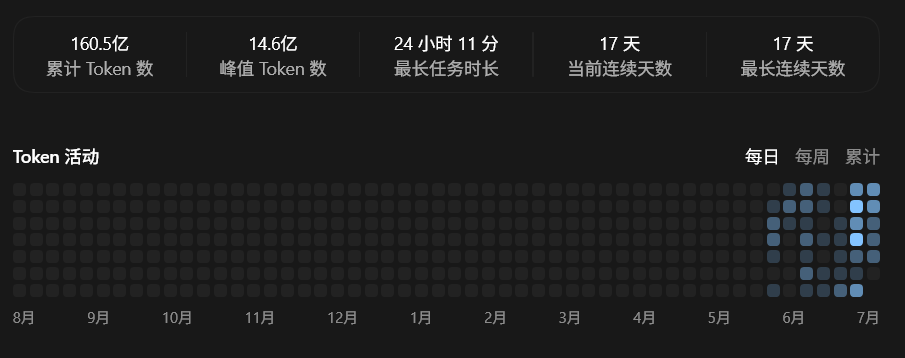
\includegraphics[width=0.96\linewidth]{token-activity.png}}
  \caption{用户提供的个人 AI 使用面板截图。面板显示累计 Token 数 160.5 亿、峰值 Token 数 14.6 亿、最长任务时长 24 小时 11 分钟，当前连续天数与最长连续天数均为 17 天。该图只反映平台统计口径下的账户使用规模，不区分工作区，也不衡量工程质量。}
  \label{fig:token-activity}
\end{figure}

这张图能直接说明的只有这一时期的 AI 使用强度；检索、生成、复核和重复实验究竟对工程产生了什么作用，仍要由 task-run、Ubuntu 日志、Yosys 输出、失败回退和哈希绑定来说明。因而，160.5 亿 Token 是投入规模的旁证，不是能力、产出或质量的替代指标。

\begin{recordnote}
\taskpath{.github/task-runs/2026-07-11-rv64-200mhz-program/task-report.md}；
\taskpath{.github/task-runs/2026-07-15-rv64-ppa-architecture-recovery/task-report.md}；
\taskpath{.github/task-runs/2026-07-22-rv64-v9i-ifu-access-current-design/task-report.md}。
\end{recordnote}

\section{回头看：模型升级只解释了一半}

\begin{table}[htbp]
  \centering
  \small
  \caption{四个月的模型、项目与协作方式}
  \begin{tabularx}{\linewidth}{@{}C{11mm}L{31mm}YYY@{}}
    \toprule
    时间 & 同期记录中的模型或执行端 & 代表项目与结果 & AI 主要承担的工作 & 当时补充的工程条件 \\
    \midrule
    4 月 & Copilot 后转 Codex
      & RV32I、NPC/DPI、trace；lint 与最小程序闭环
      & 多文件局部实现，仍依赖我搬运上下文
      & trace、batch、确定退出、Kconfig、统一入口 \\
    5 月 & Codex；GPT-5.5
      & Cache 21/21、SoC/RV64/OoO；CPI 候选与回退
      & 跨模块协议、候选实现和设计空间搜索
      & 模块回归、同口径基线、失败撤回 \\
    6 月 & Codex 与分角色 agent；部分任务记录为 GPT-5.5
      & Linux 长链、DB-first、e2e；投机失败后安全复原
      & 有界召回、图任务、验证与持久化
      & profile、manifest、task-run、Reviewer/Inspector \\
    7 月 & Codex/GPT-5 系列；同期个人记录以 GPT-5.6 Sol 为主，阶段性使用 Claude Fable 5
      & 综合/STA、架构门、负向 RTL 变体
      & 同时生成设计、测试、反例和证据验证器
      & design-id、资格门、fail-closed 发布与反证 \\
    \bottomrule
  \end{tabularx}
\end{table}

只看四月和七月的输出，确实很容易把差异全部归到模型升级上。但这几个月里，工作区本身也发生了很大变化：它开始明确告诉 AI 要读什么、允许做什么、怎样判断成功、失败后从哪里恢复，以及结果应该保存在哪里。第二部分就从这些具体结构展开。

\newarticlepart{二、现状}

\section{现在的工作区是怎么组织的}

\subsection{三层结构：Database、Skill 和 Agent}

当前工作区把 AI 相关内容分成 Database、Skill 和 Agent 三层。Database 保存可以长期保留和检索的事实，不只指某一个数据库文件；Skill 是可复用的操作规程；Agent 负责把用户目标转换成上下文、执行节点、工具动作和证据。这样划分以后，长期事实、通用做法和某次任务的执行逻辑不会混在一起。

\begin{table}[htbp]
  \centering
  \small
  \caption{当前 AI 环境的三层职责}
  \label{tab:ai-three-layer}
  \begin{tabularx}{\linewidth}{@{}L{24mm}L{38mm}YY@{}}
    \toprule
    层 & 主要入口 & 保存什么 & 不负责什么 \\
    \midrule
    Database
      & \taskpath{.github/memory/}、task-run Markdown、SQLite 索引
      & 当前状态、已知问题、历史结论、来源路径、证据索引
      & 不替代 live 源码，也不把原始大日志永久复制成“真相” \\
    Skill
      & \taskpath{.github/skills/} 与 \taskpath{SKILL.md}
      & 可复用步骤、输入输出规则、脚本入口和适用边界
      & 不决定某次任务是否完成，也不保存一次运行的全部现场 \\
    Agent
      & \taskpath{AGENTS.md}、\taskpath{AI_ENVIRONMENT.md}、instructions、profiles、runner
      & 路由任务、生成有界上下文、调度节点、执行工具、形成 task-run
      & 不可凭语言自报 PASS；完成资格由证据和发布门裁决 \\
    \bottomrule
  \end{tabularx}
\end{table}

\textbf{工程记忆（memory）}保存压缩后的稳定结论，\textbf{任务运行记录（task-run）}保留某一次执行的上下文、节点、日志和报告。前者方便下一次快速恢复状态，后者用来回答“当时到底跑了什么”。两者都不能替代 live 源码；实现是否存在，最后仍要回到当前文件确认。

\begin{figure}[htbp]
  \centering
  \resizebox{0.95\linewidth}{!}{%
  \begin{tikzpicture}[
    main/.style={draw=black,rounded corners=1.2pt,minimum width=.78\linewidth,
      minimum height=13mm,align=center,font=\small,inner sep=5pt},
    flow/.style={-{Latex[length=2.2mm]},thick},
    back/.style={-{Latex[length=2.2mm]},thick,dashed}
  ]
    \node[main] (intent) {\textbf{用户目标}\quad 自然语言需求、改动路径、期望结果};
    \node[main,below=5mm of intent] (agent) {\textbf{Agent 层}\quad
      AGENTS / AI\_ENVIRONMENT / instructions / profile / runner\\
      召回上下文，路由任务，限定动作，展开节点};
    \node[main,below=5mm of agent] (skill) {\textbf{Skill 层}\quad
      把任务转换成可复用合同、脚本和领域操作规程};
    \node[main,below=5mm of skill] (eng) {\textbf{工程执行面}\quad
      RTL、配置、仿真、综合、STA、原始日志};
    \node[main,below=5mm of eng] (evidence) {\textbf{证据链}\quad
      task-run / manifest / evidence index\quad 整理日志、报告与哈希};
    \node[main,below=5mm of evidence] (db) {\textbf{Database 层}\quad
      memory / task-run Markdown / SQLite 索引\quad 保存并检索可复核事实};
    \draw[flow] (intent) -- node[right,font=\scriptsize]{目标与边界} (agent);
    \draw[flow] (agent) -- node[right,font=\scriptsize]{调用} (skill);
    \draw[flow] (skill) -- node[right,font=\scriptsize]{执行工程动作} (eng);
    \draw[back] (eng) -- node[right,font=\scriptsize]{采集原始结果} (evidence);
    \draw[back] (evidence) -- node[right,font=\scriptsize]{发布并索引} (db);
    \draw[back] (db.west) .. controls +(-22mm,0) and +(-22mm,0) ..
      node[left,font=\scriptsize,align=right]{有界事实\\下一轮召回} (agent.west);
  \end{tikzpicture}}
  \caption{当前 AI 环境中的控制、上下文与证据回流。Database 向 Agent 提供有界事实，Skill 把 Agent 的任务转成工程动作，执行结果再经证据链回写；Database 不直接执行工程命令。}
  \label{fig:ai-three-layer}
\end{figure}

\subsection{一项任务里同时存在三条流}

项目早期经常出现一种混淆：命令确实执行了，但我问“任务是否完成”时，AI 会直接把退出码当成结论。这个问题既可能来自模型，也可能来自我没有把要求说清。后来我把一项任务拆成三条流分别记录：

\begin{table}[htbp]
  \centering
  \small
  \caption{控制流、工程数据流与证据流}
  \label{tab:three-flows}
  \begin{tabularx}{\linewidth}{@{}L{22mm}L{38mm}Y Y@{}}
    \toprule
    流 & 它回答的问题 & 主要路径 & 终点 \\
    \midrule
    控制流
      & 下一步由谁决定；失败后是否继续
      & 用户目标 $\rightarrow$ 规则路由 $\rightarrow$ profile 展开 $\rightarrow$ 节点调度
      & PASS、FAIL、BLOCKED 或 GAP \\
    工程数据流
      & 源码、配置和事务如何进入工具
      & RTL/配置 $\rightarrow$ 仿真或 EDA $\rightarrow$ 波形、网表、指标
      & 工程行为和测量值 \\
    证据流
      & 结果怎样与本次输入绑定
      & 原始日志 $\rightarrow$ report/manifest $\rightarrow$ evidence index $\rightarrow$ 发布事务
      & 可复查、可查询的 task-run \\
    \bottomrule
  \end{tabularx}
\end{table}

例如，Verilator 返回 0，只说明那条命令正常结束。它没有说明日志是否对应当前 RTL，也没有说明测试是否覆盖了这次修改。为了把结果写进 task-run，我还要核对输入身份、命令、退出码、原始日志、报告、哈希和发布状态。

\textbf{哈希（hash）}可以把文件内容压成一个数字指纹，内容发生变化，SHA-256 通常也会改变。\textbf{design-id}是针对生产 RTL 闭包计算的身份，和 Git commit 不是一回事：只改验证脚本时，Git 提交会变而 design-id 可以不变；反过来，工作树里的 RTL 尚未提交时，Git HEAD 也不能代表眼前这份实现。

\section{一项任务如何变成可追溯的 task-run}

\subsection{入口与有界上下文}

一项任务首先经过 \taskpath{AGENTS.md} 和 \taskpath{AI_ENVIRONMENT.md}。通用规则约束工作方式，模块 instructions 和 memory 提供领域背景，profile 决定要运行哪些节点。随后 runner 从任务名 \texttt{task\_slug} 里提取最多 8 个有效领域词，用这些词调用索引，生成 bounded brief。

\textbf{bounded brief} 是带 Token 上限的启动上下文包。它至少要包含三类材料：全局 canonical 规则、当前 profile 对应的领域材料，以及与本次目标直接相关、且不来自历史 task-run 的独立 focus。最后一项用来防止任务只围着旧记录打转；即使节点都能执行，也要确认模型确实看到了当前源码或当前问题。

\noindent\begin{minipage}{\linewidth}
\begin{lstlisting}[language=bash,firstnumber=1426,
  caption={启动前生成 bounded brief 的真实控制条件},
  label={code:brief-generation}]
if brief_term_text=$(e2e_context_brief_terms "$E2E_TASK_SLUG") &&
   [[ -n $brief_term_text ]]; then
  mapfile -t brief_terms <<< "$brief_term_text"
fi
if [[ ${#brief_terms[@]} -gt 0 ]] &&
   [[ ${E2E_LIVE_INDEX_REFRESH_OK:-1} = 1 ]] &&
   python3 scripts/github_index_db.py brief "${brief_terms[@]}" \
     --profile "$E2E_PROFILE" \
     --focus-scope non-history \
     --max-tokens "$max_tokens" > "$temp_brief" 2>&1; then
  generation_ok=1
fi
\end{lstlisting}
\end{minipage}

这段逻辑可以拆成六步：

\begin{enumerate}
  \item 从任务名提取领域词；提取失败时，不用空关键词继续猜。
  \item 把每个词放入数组，避免整句被当成一个不可匹配的字符串。
  \item 要求关键词数组非空。
  \item 要求 live 索引刷新成功，防止沿用过期规则。
  \item 显式传入 profile 和 \texttt{non-history} 作用域。
  \item 只有命令返回成功，临时文件才有资格成为 \taskpath{context-brief.md}。
\end{enumerate}

如果缺少 canonical、profile、独立 focus，或 Token 预算放不下必需材料，brief 会直接失败。runner 仍可继续收集诊断信息，但本轮 overall status 不会转成成功。这里采用的是\textbf{失败关闭（fail-closed）}：材料不够时保留失败状态，不用默认值把流程硬凑成绿色。

\subsection{profile 如何展开}

profile 文件的扩展名虽然是 \texttt{.tsv}，当前实现实际用竖线 \texttt{|} 分隔六个字段：

\begin{center}
\texttt{node\_id | module | function | owner\_agent | inputs | outputs}
\end{center}

\begin{table}[htbp]
  \centering
  \small
  \caption{profile 六个字段及其用途}
  \begin{tabularx}{\linewidth}{@{}L{26mm}Y Y@{}}
    \toprule
    字段 & 通俗解释 & 为什么需要 \\
    \midrule
    \texttt{node\_id} & 节点的唯一名字 & 让日志、报告和失败位置可被稳定引用 \\
    \texttt{module} & 节点所属领域；include 行中表示另一个 profile & 支持组合与复用 \\
    \texttt{function} & 真正执行的 shell 函数 & 配置必须落到可运行实现，而不是口号 \\
    \texttt{owner\_agent} & 对结论负责的角色 & 区分实现、工具链、硬件流等责任 \\
    \texttt{inputs} & 节点声明读取的文件或能力 & 让输入边界可审计 \\
    \texttt{outputs} & 预期证明的结果 & 让“为什么通过”可解释 \\
    \bottomrule
  \end{tabularx}
\end{table}

当前 \taskpath{.github/e2e/profiles/agent-system.tsv} 只有 8 个物理行，却同时承担发现、合同、状态回溯和交付审计。逐行展开它，最能看清这套环境怎样从文档约定落到可执行节点。

\noindent\begin{minipage}{\linewidth}
\begin{lstlisting}[language={},basicstyle=\ttfamily\zihao{6},
  caption={\texttt{agent-system.tsv} 的当前 8 行配置},
  label={code:agent-system-profile}]
@include|discovery||||
three-layer-contract|agent-system|e2e_agent_system_three_layer_contract|agent-system|AI_ENVIRONMENT.md;.github/instructions/agent-env-layer-contract.instructions.md;.github/skills/agent-env-maintenance/SKILL.md;scripts/agent-maintain.sh|验证一页导航、canonical 路径与 Database/Skill/Agent 三层契约
runtime-artifact-boundary|agent-system|e2e_agent_system_runtime_artifact_boundary|agent-system|.github/ai-env/contracts/agent-env-runtime-artifacts.json;.github/ai-env/contracts/agent-env-policy.json;scripts/agent-maintain.sh|验证源码面与运行态 artifact/store 分层边界
state-machine-traceback|agent-system|e2e_agent_system_state_traceback|agent-system|.github/instructions/agent-env-state-machine.instructions.md;.github/ai-env/contracts/agent-env-state-traceability.json;scripts/e2e/lib/report.sh|验证状态机回退和 task-run state_traceback 字段
reviewer-inspector-gate|agent-system|e2e_agent_system_reviewer_inspector_gate|agent-system|.github/ai-env/contracts/agent-env-review-routing.json;.github/ai-env/contracts/agent-env-policy.json;.github/e2e/profiles/agent-system.tsv|验证 Reviewer/Inspector 路由已落成 profile 执行节点
rtl-task-contract|agent-system|e2e_agent_system_rtl_task_contract|agent-system|.github/ai-env/contracts/agent-env-rtl-task-contract.json;.github/instructions/rtl-agent-task-contract.instructions.md;.github/skills/prepare-rtl-task-contract/SKILL.md;.github/skills/prepare-rtl-task-contract/scripts/rtl_task_contract.py|验证本地 RTL 子任务契约可生成、校验、渲染并拒绝越权 mutation
commercial-delivery-readiness|agent-system|e2e_agent_system_commercial_delivery_readiness|agent-system|.github/ai-env/contracts/agent-env-delivery.json;deliverables/ai-dev-env-commercial-v1;scripts/package-ai-dev-env.sh|验证商业交付包装、旧产物归档和 delivery audit
profile-index|agent-system|e2e_agent_system_profile_index|agent-system|.github/e2e/profiles|列出所有可执行 profile
\end{lstlisting}
\end{minipage}

\begin{longtable}{@{}C{9mm}L{31mm}L{50mm}L{50mm}@{}}
  \caption{\texttt{agent-system.tsv} 逐行解释}
  \label{tab:agent-system-line-by-line}\\
  \toprule
  行 & 配置项 & 这一行实际做什么 & 输入、输出与失败后果 \\
  \midrule
  \endfirsthead
  \multicolumn{4}{c}{续表：\texttt{agent-system.tsv} 逐行解释}\\
  \toprule
  行 & 配置项 & 这一行实际做什么 & 输入、输出与失败后果 \\
  \midrule
  \endhead
  \bottomrule
  \endfoot
  1 & \texttt{@include discovery}
    & 递归插入基础发现 profile；include 本身不是执行节点。
    & 输入是 \taskpath{discovery.tsv}；先展开 3 个节点。解析失败则整个 profile 无法调度。 \\
  2 & \path{three-layer-contract}
    & 检查一页入口、canonical 路径，以及 Database/Skill/Agent 三层是否真的接通。
    & 读取导航、三层合同、维护 skill 和脚本；输出同名节点日志。 \\
  3 & \path{runtime-artifact-boundary}
    & 检查 tracked source、运行时临时产物和数据库索引之间的边界。
    & 防止把临时 payload 当长期源码，也防止把大日志全文塞进长期数据库。 \\
  4 & \path{state-machine-traceback}
    & 检查任务状态能否从最终结果回溯到节点、输入和 rollback target。
    & 输出必须包含可验证的 \texttt{state\_traceback}；缺字段即失败。 \\
  5 & \path{reviewer-inspector-gate}
    & 检查 Reviewer 与 Inspector 不是文档称谓，而是 profile 中真实可执行的审查节点。
    & 读取路由合同和 policy；实现者自报不能替代独立审查。 \\
  6 & \path{rtl-task-contract}
    & 自测 RTL 子任务合同能否创建、校验和渲染，并拒绝未授权的 mutation。
    & 输入包括合同 JSON、instruction、skill 和脚本；越权动作必须成为负例。 \\
  7 & \path{commercial-delivery-readiness}
    & 检查交付源、旧产物归档、打包和 delivery audit。
    & 它证明包装流程可运行，不等于某个 RV64 技术目标已经闭合。 \\
  8 & \texttt{profile-index}
    & 枚举所有 profile，确认入口能够发现它们。
    & 输入是 profile 目录；遗漏或格式错误会使索引节点失败。 \\
\end{longtable}

第一行之所以会展开，是因为加载器会递归处理 \texttt{@include}：

\noindent\begin{minipage}{\linewidth}
\begin{lstlisting}[language=bash,firstnumber=180,
  caption={profile 的深度优先 include 逻辑},
  label={code:profile-include}]
IFS='|' read -r node module function owner inputs outputs
if [[ $node = "@include" ]]; then
  load_profile "$module"
  continue
fi
\end{lstlisting}
\end{minipage}

代码清单先用 \texttt{IFS='|'} 把一条配置拆成六个字段；若 \texttt{node} 为 \texttt{@include}，加载器便递归读取 \texttt{module} 字段指定的 profile，再跳过当前 include 行。因此，\texttt{agent-system.tsv} 表面上只有 8 行，展开后实际包含 10 个节点。

\taskpath{discovery.tsv} 会先展开三个前置节点：

\begin{enumerate}
  \item \texttt{recall-discovery}：确认 AGENTS、instructions、memory、profiles 和脚本入口存在；
  \item \texttt{tool-env-check}：检查 bash、git、make、Python、gcc、Verilator 等工具可见；
  \item \texttt{npc-sim-status}：读取 NPC/sim backend 状态，但不因此证明 NPC 功能正确。
\end{enumerate}

按照深度优先方式展开后，完整顺序如下：

\begin{center}
\small
\texttt{recall-discovery $\rightarrow$ tool-env-check $\rightarrow$ npc-sim-status}\\
\texttt{$\rightarrow$ three-layer-contract $\rightarrow$ runtime-artifact-boundary}\\
\texttt{$\rightarrow$ state-machine-traceback $\rightarrow$ reviewer-inspector-gate}\\
\texttt{$\rightarrow$ rtl-task-contract $\rightarrow$ commercial-delivery-readiness}\\
\texttt{$\rightarrow$ profile-index}
\end{center}

每个节点的原始日志统一写入
\taskpath{.github/task-runs/<run_id>/evidence/<node_id>.log}。
\taskpath{nodes.tsv} 保存展开后的节点表，\taskpath{dispatch-log.md} 记录调度过程；我排查具体结果时，最终依据仍是节点日志。

\subsection{从执行到发布的 12 个阶段}

\begin{longtable}{@{}C{8mm}L{24mm}L{39mm}L{30mm}L{35mm}@{}}
  \caption{一次 workflow 从输入到发布的 12 个阶段}
  \label{tab:workflow-twelve-steps}\\
  \toprule
  步 & 输入 & 处理 & 输出 & 失败分支 \\
  \midrule
  \endfirsthead
  \multicolumn{5}{c}{续表：一次 workflow 从输入到发布的完整数据流}\\
  \toprule
  步 & 输入 & 处理 & 输出 & 失败分支 \\
  \midrule
  \endhead
  \bottomrule
  \endfoot
  1 & 用户目标、修改路径
    & 读取入口规则，选择领域 profile
    & profile 名称、任务约束
    & 无匹配领域或入口缺失时停止 \\
  2 & \texttt{task\_slug}
    & 去噪，保留最多 8 个领域词
    & 召回关键词
    & 无领域词、修订标签畸形或重复时失败 \\
  3 & live 索引、canonical、profile、focus
    & 生成并验证 bounded brief
    & \taskpath{context-brief.md}
    & 缺独立 non-history focus 或超预算时失败 \\
  4 & profile TSV
    & 递归展开 \texttt{@include}
    & \taskpath{profile-resolve.md}
    & include 循环、缺函数或格式错误时停止 \\
  5 & brief、闭包、节点输入
    & 逐节点调用绑定函数
    & \taskpath{evidence/*.log}、\taskpath{nodes.tsv}、dispatch
    & required 节点 FAIL/SKIP 时不能 completed \\
  6 & 节点状态与证据引用
    & 生成人读报告和机读清单
    & \taskpath{task-report.md}、\taskpath{run-manifest.json}
    & 状态、身份或节点集合不一致时失败 \\
  7 & 普通日志与唯一 manifest
    & 计算大小、行数、SHA-256 并入索引
    & \taskpath{evidence-index.md}、DB \path{evidence_assets}
    & symlink、重复身份或索引缺项时失败 \\
  8 & 七项关键产物
    & 计算并绑定产物哈希
    & \taskpath{complete.marker}
    & 任一产物缺失或哈希不一致时失败 \\
  9 & task-run Markdown
    & 同步到数据库暂存集合
    & staged DB records
    & live 与 staged 内容不同则删除候选 marker \\
  10 & marker 与任务身份
    & 写发布声明
    & \taskpath{completion-publication.md}
    & profile、run-id 或哈希不一致时失败 \\
  11 & 文件快照与 staged DB
    & SQLite \texttt{BEGIN IMMEDIATE} 原子复核并提交
    & \texttt{db-marker-v1} publication
    & 任一文件在事务中变化则整体回滚 \\
  12 & 修改路径、语义时间、已发布 run
    & strict guard 检查覆盖与新鲜度
    & PASS 或明确缺口
    & 旧证据、错 profile 或未发布 run 均拒绝 \\
\end{longtable}

\textbf{manifest} 是机器可读的产物清单；\textbf{state traceback} 用来从最终状态追到节点、输入、证据和回滚点；\textbf{evidence index} 只记录证据文件的路径、大小和哈希，不把原始 payload 全文复制进长期记忆。

\subsection{marker 为什么只代表候选完成}

\taskpath{complete.marker} 绑定七项基础产物：

\begin{center}
\small
\taskpath{task-report.md}、\taskpath{run-manifest.json}、\taskpath{context-brief.md}、\\
\taskpath{profile-resolve.md}、\taskpath{evidence-index.md}、\taskpath{dispatch-log.md}、\taskpath{nodes.tsv}。
\end{center}

旧说明文档曾把顺序写成“先 staged archive，再 marker”，当前实现实际按下面的顺序执行：

\begin{center}
\texttt{validate bundle $\rightarrow$ complete.marker $\rightarrow$ staged archive}\\
\texttt{$\rightarrow$ completion-publication $\rightarrow$ atomic DB publication}
\end{center}

写入 marker 之后，如果暂存归档或发布校验失败，代码会主动删除 marker 和 publication。因此 marker 只表示“这份 bundle 已经通过初步校验”，还不是最终完成。查询接口只把带有效 \texttt{db-marker-v1} publication 的 run 计为 completed。

\noindent\begin{minipage}{\linewidth}
\begin{lstlisting}[language=Python,firstnumber=1868,
  caption={数据库发布用一个事务重新检查文件与暂存内容},
  label={code:atomic-publication}]
conn.execute("BEGIN IMMEDIATE")
for name, raw in snapshot.items():
    if read_ordinary(name) != raw:
        raise ValueError(
            f"artifact changed during publication: {name}")
if stored != staged_markdown:
    raise ValueError(
        "staged DB Markdown set or content changed before publication")
...
conn.commit()
\end{lstlisting}
\end{minipage}

这里的\textbf{数据库事务（transaction）}与硬件里的 transaction 同名，但用途不同。它保证多项数据库更新要么一起提交，要么一起回滚。发布期间如果文件被修改、暂存集合发生变化，或已有记录冲突，整次发布都会撤销，不留下半完成状态。

\subsection{strict guard 检查什么}

\textbf{strict guard} 放在流程末尾。它根据修改路径推导需要哪些 profile，并检查相应证据是否完整、已发布、且时间上足够新。文件系统的 \texttt{mtime} 可以用 \texttt{touch} 改掉，但任务的语义完成时间、发布身份和 evidence bundle 不能靠改时间戳伪造。

这套机制已经抓到过几类实际问题：

\begin{itemize}
  \item 5/5 节点 PASS，却没有独立 non-history focus；系统拒绝发布；
  \item state traceback 验证器把 \texttt{run\_id} 当作 \texttt{run\_root}，且 evidence index 漏掉顶层 manifest；修复后分别检查普通证据和唯一 manifest；
  \item canonical evidence 生成后又追加 dispatch/review provenance，旧证据立刻变成 freshness GAP；正确做法是冻结记录后重放叶证据与上层聚合；
  \item PowerShell 提前展开 Bash 的 \texttt{\$var}，或多个 WSL 命令并发占用同一工程，会造成“看似脚本失败”的环境假故障；我后来只把 PowerShell 当作 \texttt{wsl.exe} 启动器，并让工程 shell 保持 single-flight（同一时刻只允许一条执行链占用工程）。
\end{itemize}

\textbf{single-flight} 指同一时刻只允许一个主体占用工程 shell。它与 RTL 性能无关，主要用来避免两个 agent 同时改配置、复用同一个 build 目录或争抢仿真状态。不同角色仍可并行分析，但实际工程命令按所有权串行执行。

\begin{boundarynote}
节点 PASS 表示对应检查按合同执行完成；task-run completed 表示这次证据链已经成功发布。它们描述的是流程状态，不直接等同于 RV64 Core 的功能、架构或 PPA 目标。涉及 RTL 的结论仍要看相应的技术证据。
\end{boundarynote}

\section{以一次 FENCE 任务为例}

下面用 7 月 23 日的一次普通 FENCE 任务把三条流串起来。FENCE 是 RISC-V 的内存顺序指令，它要求指定范围内的早期访存先完成，后续访存才能继续。实现时不能简单写成“固定等几拍”，而要等待相关内存状态真正清空。

\begin{longtable}{@{}C{8mm}L{25mm}L{39mm}L{29mm}L{35mm}@{}}
  \caption{普通 FENCE 任务中的控制流、工程数据流和证据流}
  \label{tab:fence-task-flow}\\
  \toprule
  步 & 输入 & 动作 & 输出 & 失败时怎样处理 \\
  \midrule
  \endfirsthead
  \multicolumn{5}{c}{续表：普通 FENCE 任务的三类数据流}\\
  \toprule
  步 & 输入 & 动作 & 输出 & 失败时怎样处理 \\
  \midrule
  \endhead
  \bottomrule
  \endfoot
  1 & older store、FENCE、younger device read 必须有序
    & 入口判定为 RV64 RTL 与 npc-dev 领域
    & 需要的规则、profile 和成功条件
    & 不允许退化成只改 testbench 的模糊任务 \\
  2 & \texttt{fence ordering} 领域词
    & bounded recall 读取 NPC memory、架构合同和非历史源码片段
    & 与 FENCE、memory owner、drain 相关的有限上下文
    & 缺独立 focus 时 brief 失败 \\
  3 & task contract
    & 固定生产 RTL、testbench、命令、负向版本和证据路径
    & 明确“什么能改、什么不能改、怎样算成功”
    & 子任务越权修改生产 RTL 时拒绝 \\
  4 & 当前模块与信号
    & 追踪 \texttt{mem\_idle\_o} 从后端到控制面的连线
    & 完整调用链和漏接风险
    & 任何一层常量化或错接都进入负向故障模型 \\
  5 & STORE、FENCE 与设备读程序
    & 仿真 older store 的 probe/drain、FENCE 等待和年轻读
    & focused 2/2
    & FENCE 提前退休或年轻读提前出现即 FAIL \\
  6 & 当前模块清单
    & 运行模块 aggregate
    & 109/109
    & 缺项、重复项、编译/仿真 rc 异常均拒绝 \\
  7 & 两个临时错误 RTL
    & 分别切断 FENCE 的 \texttt{mem\_idle} 条件和 CoreGlue 连线
    & 2/2 可编译，且都被目标 checker 精确拒绝
    & 错误版本若通过，说明测试是假绿 \\
  8 & 原始日志与当前 design-id
    & 证据验证器检查唯一失败 marker、哈希、来源和绑定
    & validator unit 12/12
    & 自报 JSON、模糊前缀或旧日志不能替代原始失败 \\
  9 & 受共享文件影响的架构门
    & 重放 9 个 canonical directed gates 与 arch-stable audit
    & 9 门 GREEN；freeze 仍为 GAP
    & 不只改 ledger 哈希；必须重跑受影响证据 \\
  10 & task-run、memory
    & 冻结 provenance，再发布记录
    & 下一次任务可按 FENCE 和 design-id 召回
    & 后置字节变化会让旧证据变 stale \\
\end{longtable}

在这项任务里，控制流负责决定下一步运行什么，工程数据流让 STORE、FENCE 和 device read 真正穿过 RTL，证据流则把结果绑定到 design-id、负向版本和 task-run。三条记录需要相互对得上，才能把 \texttt{FENCE-G1=CLOSED} 写进当前快照。

\begin{recordnote}
\taskpath{.github/memory/modules/npc.md} 中的 “RV64 ordinary FENCE current-design V9M”；
\taskpath{.github/memory/project-status.md} 的 2026-07-23 FENCE-G1 条目。
\end{recordnote}

\section{当前 RV64 Core 的基本结构}

\subsection{从指令集到微操作}

\textbf{RISC-V} 是一套开放指令集架构；\textbf{RV64} 表示通用整数寄存器和主要地址宽度为 64 位。指令集架构（Instruction Set Architecture，ISA）规定软件能看见的寄存器、指令、异常和内存语义，RTL 则规定这些语义怎样由电路实现。

最近已验证的生产快照覆盖 RV64IMAFDC、Zicsr、Zba/Zbb/Zbc/Zbs，并实现 M/S/U 特权级、Sv39、I/D TLB、硬件页表遍历和 16 个 PMP 条目。下面先解释几项后文会反复出现的缩写：

以下关于功能范围、结构和容量的叙述，以最近已验证的生产快照为基准；明确标为“live 工作树”的代码只用于解释当前接口合同，不能继承该快照的测试数字。

\begin{itemize}
  \item \textbf{Sv39}：RISC-V 的 39 位虚拟地址分页方案；
  \item \textbf{TLB（Translation Lookaside Buffer）}：缓存虚拟地址到物理地址的翻译；
  \item \textbf{PTW（Page Table Walker）}：TLB miss 时读取多级页表的硬件状态机；
  \item \textbf{PTE（Page Table Entry）}：页表项，保存物理页号和访问权限；
  \item \textbf{PMP（Physical Memory Protection）}：按物理地址检查读、写、执行权限；
  \item \textbf{CSR（Control and Status Register）}：特权控制和状态寄存器。
\end{itemize}

指令进入后端后，会被表示成\textbf{微操作（micro-operation，uop）}。其中携带 PC、原始指令、源/目标寄存器、立即数、ROB 编号、物理寄存器号和异常字段。当前实现仍通过多组分散端口传递这些信息，还没有收敛成统一的 \texttt{uop\_t}；旧的 50-bit \texttt{CTRL\_BUS} 也继续被 OoO 路径复用，维护成本已经比较明显。

\subsection{“乱序执行、顺序退休”是什么意思}

\textbf{乱序执行（Out-of-Order，OoO）}允许较新的、已经就绪的指令先于被阻塞的老指令执行，以减少执行单元空等。但结果仍按程序顺序退休，这样软件看到的状态才与顺序执行语义一致。

它依赖几类核心结构：

\begin{itemize}
  \item \textbf{ROB（Reorder Buffer，重排序缓冲区）}：按程序顺序保存 uop，记录完成、结果和异常；当前深度 16；
  \item \textbf{RAT（Register Alias Table，寄存器重命名表）}：把架构寄存器映射到物理寄存器，消除名字相同造成的假依赖；
  \item \textbf{PRF（Physical Register File，物理寄存器堆）}：保存投机执行结果；整数与浮点各 64 项；
  \item \textbf{IQ（Issue Queue，发射队列）}：保存尚未发射的 uop，从中选择操作数已就绪且执行资源可用者；整数与浮点各 8 项；
  \item \textbf{SQ（Store Queue，存储队列）}：保存 store 的地址、数据、所有权和提交后排水状态；当前 4 项；
  \item \textbf{MIQ（Memory Inflight Queue，内存在途队列）}：保存 load、probe 和 drain 等内存运输事件；当前 4 项。
\end{itemize}

\begin{figure}[htbp]
  \centering
  \resizebox{0.98\linewidth}{!}{%
  \begin{tikzpicture}[
    block/.style={draw=black,rounded corners=1pt,minimum width=27mm,
      minimum height=12mm,align=center,font=\small,inner sep=4pt},
    smallblock/.style={draw=black,minimum width=23mm,minimum height=9mm,
      align=center,font=\scriptsize,inner sep=3pt},
    flow/.style={-{Latex[length=2.0mm]},thick},
    feedback/.style={-{Latex[length=2.0mm]},dashed}
  ]
    \node[block] (fetch) {取指与预测\\IFU / fetch packet};
    \node[block,right=7mm of fetch] (rename) {译码与重命名\\RAT / FreeList};
    \node[block,right=7mm of rename] (rob) {分配\\ROB16 + IQ8};
    \node[block,right=7mm of rob] (issue) {唤醒与发射\\oldest-ready};
    \node[block,right=7mm of issue] (exec) {执行簇\\INT / FP / BR / MEM};
    \node[block,right=7mm of exec] (wb) {写回\\PRF + ROB done};
    \node[block,right=7mm of wb] (commit) {顺序退休\\架构 GPR/CSR};
    \draw[flow] (fetch) -- (rename);
    \draw[flow] (rename) -- (rob);
    \draw[flow] (rob) -- (issue);
    \draw[flow] (issue) -- (exec);
    \draw[flow] (exec) -- (wb);
    \draw[flow] (wb) -- (commit);
    \draw[feedback] (wb.south) .. controls +(0,-13mm) and +(0,-13mm) ..
      node[below,font=\scriptsize]{完成广播唤醒依赖者} (issue.south);
    \node[smallblock,below=25mm of exec] (mem) {双 memory bridge\\DTLB/PTW/PMP/D-cache};
    \node[smallblock,right=7mm of mem] (axi) {共享原始 AXI\\miss/PTW/store 排队};
    \draw[flow] (exec) -- (mem);
    \draw[flow] (mem) -- (axi);
    \node[smallblock,below=25mm of rob] (control) {Control Plane\\trap/redirect/drain};
    \draw[feedback] (commit) |- (control);
    \draw[feedback] (control) -| node[below,font=\scriptsize]{redirect / flush} (fetch);
  \end{tikzpicture}}
  \caption{当前 RV64 Core 的主数据通路。图示为职责关系，省略大量 wrapper 与散线。}
  \label{fig:rv64-main-flow}
\end{figure}

\subsection{一条普通整数指令怎样流动}

\begin{enumerate}
  \item \textbf{取指。}取指桥对 PC 做 TLB、PTW、PMP 和 AXI 访问，形成双槽 fetch packet。预测器给出下一 PC。
  \item \textbf{译码。}指令被解释为操作类型、源寄存器、目标寄存器和立即数。
  \item \textbf{重命名。}RAT 给源操作数找到物理寄存器，FreeList 为目标分配新物理寄存器；旧映射被保存，供退休释放或恢复。
  \item \textbf{分配。}同一 uop 进入 ROB 与 IQ。ROB 保存程序顺序，IQ 等待操作数和执行资源。
  \item \textbf{发射。}调度器在已就绪 uop 中选择最老者，当前整数主路径可双发射。
  \item \textbf{执行与写回。}ALU、乘除、位操作、分支、浮点或 memory 单元产生 result event；PRF 写入结果，ROB 标记完成，并广播唤醒依赖者。
  \item \textbf{退休。}只有 ROB 头部已完成且无阻塞，结果才进入架构 GPR/CSR；异常项在这里形成精确 trap，并抑制更年轻退休。
\end{enumerate}

这里的\textbf{退休（retire/commit）}指结果正式进入架构状态、对软件可见，与“执行单元已经算完”不是同一件事。第 10 条指令可以先完成计算，但只要前面的老指令还没有满足退休条件，它就不能越过这些指令修改架构状态。

\subsection{为什么仍然保留两个执行域}

当前设计把高频 branch/jump、整数、FP、load/store/AMO 放在 OoO 域 A：

\begin{center}
\texttt{fetch $\rightarrow$ rename $\rightarrow$ ROB/IQ $\rightarrow$ issue $\rightarrow$ execute $\rightarrow$ writeback $\rightarrow$ commit}
\end{center}

system、trap、IRQ 和 fault 目前默认走域 B：先记录 pending，停止继续派发，等待 ROB、IQ、SQ 和 memory owner 排空，再交给控制面处理并恢复取指。这样做会损失一部分并行度，但精确性更容易控制。它只是对少数高风险事件做串行化，并不意味着整个核心按顺序执行。后续若改成 serialize-at-retire，需要逐项重建相应证明，不能只为了 IPC 一次性放开。

\subsection{握手、反压和 transaction}

硬件接口常用 \texttt{valid}/\texttt{ready} 握手。发送方把 \texttt{valid} 拉高，表示当前 payload 有效；接收方把 \texttt{ready} 拉高，表示这一拍可以接收。只有二者在同一个时钟沿同时为 1，这次 transaction 才算真正转移；这种同拍握手通常记作 \texttt{fire}。

\textbf{反压（backpressure）}是下游把 \texttt{ready} 拉低，要求上游保持 \texttt{valid} 和 payload 不变。反压不是错误，而是正常流控。常见错误包括：

\begin{itemize}
  \item 只看到 \texttt{valid} 就提前消费，导致同一响应丢失或重复；
  \item 等待期间改变地址、数据或 owner，导致响应归错事务；
  \item flush 后直接清空已经发出的 AXI 写，使外部副作用与内部状态分离；
  \item 用会循环复用的 ROB index 当唯一身份，年轻新指令误认旧响应。
\end{itemize}

为避免身份混淆，当前设计使用 \textbf{ProducerId} 和 owner token。ProducerId 由 ROB slot 的 generation 与 index 共同组成，token 用来索引内存 owner 表。比较两个事件时，不能只看它们是否都指向“ROB 第 3 项”，还要确认 generation、owner kind 和 MMU epoch 是否一致。

\section{RV64 Core 的几轮关键调整}

\subsection{阶段回顾}

\begin{longtable}{@{}L{20mm}L{34mm}L{50mm}L{36mm}@{}}
  \caption{从早期 OoO 骨架到最近已验证 RV64 快照}
  \label{tab:rv64-timeline}\\
  \toprule
  时间 & 当时目标与状态 & 实现变化 & 可核验证据与边界 \\
  \midrule
  \endfirsthead
  \multicolumn{4}{c}{续表：从早期 OoO 方法到最近已验证 RV64 快照}\\
  \toprule
  时间 & 当时目标与状态 & 实现变化 & 可核验证据与边界 \\
  \midrule
  \endhead
  \bottomrule
  \endfoot
  5 月 28 日
    & RV32 顺序核上的 OoO 方法学前身
    & 旁路建立 RenameMap、FreeList、ROB，不接主路径
    & 新增 TB 3/3、模块 30/30；明确“不声称完成 OoO 或 CPI 改善” \\
  5 月 29 日
    & 建立早期 OoO 闭环，长期目标 CPI=0.5
    & 修复 IQ bypass 误删；比较双 memory 与 branch+ret 候选
    & AM add 541/839、CPI=0.645；退化或组合环候选回退 \\
  5 月 30 日
    & RV64 改为 OoO-only
    & 修正 8-byte cache/AXI lane、PMEM 范围、\texttt{*W}/M/B 指令；删除顺序路由
    & CoreMark-1000 阶段 CPI 6.017 $\rightarrow$ 0.779；仍非完整功能/PPA \\
  5 月末至 6 月
    & 从“能跑”转向 owner、flush 和可维护性
    & 补 AXI drain、Sv39、特权、FP；拆分巨石模块，增加 spec 和模块 TB
    & 多个局部 gate；不能把 QEMU、NPC、Linux 路径相互替代 \\
  7 月 2—11 日
    & 高频指令进入真实 OoO 域
    & branch/jump、memory、FP 迁入 rename/IQ/ROB；FP 独立簇、issue resolve、显式 mispredict、ROB-walk
    & B2 阶段 CoreMark CPI 1.064 $\rightarrow$ 0.877；同阶段 STA WNS 仍为 $-15.37$ ns \\
  7 月 14—21 日
    & 功能、架构、时序分层
    & 补 frontend II=1、七边界双宽、双 memory、长延迟越过、选择性调度与恢复
    & DI-1 至 DI-5、OOO-1 至 OOO-4 九项定向门逐项建立 \\
  7 月 22—23 日
    & 关闭当前快照的功能与关键所有权合同
    & 分离 ROB launch/owner；约束 response credit、retry token；补 FENCE 与 STORE/AMO next-edge residency
    & design-id \texttt{2eff...c8b2}：功能集合全过、9 门 GREEN；full-core 仍 GAP，PPA 未资格化 \\
\end{longtable}

这条时间线里的性能数字不能直接排成排行榜。CPI 0.645、0.779 和 0.877 分别来自不同核心、镜像和阶段，有些数字出现时，后来的架构门还没有建立。只有输入、设计和计数范围一致时，性能比较才有意义。

\subsection{我后来固定下来的工作顺序}

后来我把每轮 RV64 优化固定成下面七步：

\begin{enumerate}
  \item \textbf{RECALL。}读取当前 ROADMAP、架构合同、模块 memory 和相关 task-run，先恢复已知边界。
  \item \textbf{CONTRACT。}在改 RTL 前冻结接口、stall、flush、异常序、访存序和恢复语义；定义 owner 与 transaction 生命周期。
  \item \textbf{IMPL。}一次只改变一个主要责任，避免把架构修复、文档更新和无关重构混在同一刀。
  \item \textbf{VERIFY。}先跑 focused 正例和负例，再运行 lint、build、module、official、AM 与适用的 Difftest；检查原始日志，不只看 summary。
  \item \textbf{PPA。}只有功能与架构硬门通过，才比较同源性能、综合和 STA；工具输出必须附模型边界。
  \item \textbf{REVIEW。}实现者交付证据，审查者主动寻找“前置条件从未被触发”造成的假通过、错误的期望结果、覆盖空洞和超出证据范围的结论。
  \item \textbf{RECORD。}更新 active spec、current snapshot、memory 和 task-run，使下一轮能直接召回成功与失败。
\end{enumerate}

这套顺序并不是先把代码写完，再补一轮测试。CONTRACT 会直接影响实现方式，VERIFY 发现的新故障又会反过来修改合同；失败方案被写进 RECORD 后，后续任务也能少走一次重复的弯路。

\subsection{一次 IQ 挂死，以及两项被撤回的实验}

\paragraph{表象}

早期 IQ 曾出现过一种挂死：某个依赖者一直等不到生产者，看起来像随机停住。与此同时，另一个放宽双 memory 的实验虽然能跑完，却把 CPI 从 0.645 拉坏到 0.665。

\paragraph{根因}

\texttt{issue0} 有时直接来自 dispatch bypass，并不占用 IQ entry；旧 compact 逻辑却无条件按默认 index 0 删除队列项。真正的 producer 被误删，消费者再也收不到完成广播。

\paragraph{实现与判断}

最终修改为：只有 issue 确实来自真实 queue 且发生 fire 时，才删除对应 entry。这个正确性修复被保留；双 memory 放宽则因为同口径性能退化而撤回。两项修改虽然发生在同一轮任务里，结论仍然分开处理。

\subsection{局部测试通过，组合环仍然存在}

branch 与 ret 同拍的候选通过了局部 testbench，但 Verilator 报出 \texttt{UNOPTFLAT}。组合环穿过 dispatch ready、branch resolve 和 lane1 valid，也就是某段组合逻辑的输出在同一拍又回到自己的输入。即使功能样例暂时能跑，这种结构仍可能造成仿真迭代、综合问题或很差的时序。

我没有再加条件把警告压下去，而是撤回了整个候选，并把跨边界的 ready/valid 依赖加入后续结构检查。局部功能测试、静态结构检查和 STA 各自覆盖不同问题，任何一项都不能替代另外两项。

\subsection{修掉硬件卡点后，又露出软件问题}

CoreMark 曾经稳定停在 \texttt{commits=325846}。先查到的是硬件问题：flush 清除了后端 pending，但 memory bridge 仍持有已经发出的 AXI response，内部 owner 与外部事务因此脱节。补齐 read/write drain 后，程序越过了这个卡点，却又暴露出 \taskpath{stdio.c} 的 RV64/Zba 指针问题：\texttt{zext.w} 把终止指针错误地截成了 32 位。

因此，“找到了 root cause”往往只对当前卡点成立。修掉第一层之后，系统可能只是继续运行到下一处问题。调试时需要保留提交计数、PC、owner 和日志差异，确认失败位置如何变化，不能因为卡点向后移动就直接把任务写成完成。

\subsection{BPU 表项没错，采样时点仍然会错}

我曾把 BPU lookup 移到 enqueue 的下一拍，随后又补了 FIFO 写回和 fill bypass。连续三轮修改后，accuracy 仍只有 78.4\%，比基线低 10.2 个百分点。探针显示预测表和回训数据本身没有明显问题，问题更可能出在 GHR（Global History Register，全局分支历史）的采样时点。

最后我把这一组修改整体回退。AI 在这轮工作的作用，是快速生成并排除多个诊断候选；当证据已经指向架构时点问题时，继续往现有补丁上叠条件只会增加复杂度。

\subsection{功能不变，PPA 仍可能变差}

删除 cross-lane current-result forward 后，focused 5/5、module 93/93，CoreMark 的周期数也与基线完全一致。单看功能结果，这很像一次干净的“删死逻辑”。但同口径的 PPA 评估给出了相反结果：

\begin{itemize}
  \item WNS 从 $-10.001$ ns 恶化到 $-10.182$ ns；
  \item TNS 恶化 18.5\%；
  \item combinational loop 报告从 109 增至 142；
  \item 面积和功耗代理值也上升。
\end{itemize}

因此这个候选被拒绝并还原。RTL 行数减少不代表网表一定更小，删掉局部 mux 也可能改变综合映射、扇出和关键路径。PPA 只能在同一套输入和工具条件下测出来，不能靠看源码猜。

\subsection{吞吐提高，也不能抵消一项官方测试失败}

R3.2 early wake 一度带来 5.3323\% 的吞吐提升，但官方测试首先掉到 176/177。根因是 \texttt{clear\_arch\_squash} 与 \texttt{capture\_arch} 同拍发生时，后写的非阻塞赋值重新激活了 wrong-path trap。修正后功能回归恢复全绿，不过 exact-5ns WNS 仍为 $-0.433356$ ns；按当时的资格门，面积效率也仍未达标，所以这一版本没有晋级。

当前 PPA 合同因此把功能、架构和时序设为硬门。吞吐提高多少，都不能抵消其中一项失败。

\begin{recordnote}
\taskpath{.github/task-runs/2026-05-29-ooo-cpi-645-iq-fix/task-report.md}；
\taskpath{.github/task-runs/2026-05-30-rv64-ooo-flush-drain-coremark/task-report.md}；
\taskpath{.github/task-runs/2026-07-11-knife-b2-s2s3/task-report.md}；
\taskpath{.github/task-runs/2026-07-13-rv64-t3a-current-top-retry/task-report.md}；
\taskpath{.github/task-runs/2026-07-15-rv64-ppa-architecture-recovery/task-report.md}。
\end{recordnote}

\section{当前实现中最关键的一件事：事务所有权}

\subsection{为什么“发射许可”和“事务所有权”不能共用一个条件}

STORE 或 AMO 只有到达 ROB head 后，才可能获得第一次物理写发射许可。发射前若处于 flush 或 recovery，应禁止产生新的外部副作用；但 AW/W 一旦已经送到 AXI，事务就不能再被内部恢复逻辑抹掉。即使核心正在清理年轻指令，这笔已经发出的写仍要保留 owner，直到收到最终 B response。

当前 live 工作树中的 \taskpath{OooRob.v} 用两个信号分别表示这两件事：

\noindent\begin{minipage}{\linewidth}
\begin{lstlisting}[language=Verilog,firstnumber=528,
  caption={ROB head 的首次发射许可与发射后所有权},
  label={code:rob-launch-owner}]
assign head0_owner_open_o = !rst &&
    (count_q != {ROB_COUNT_W{1'b0}}) &&
    valid_q[head_q] && !done_q[head_q];

assign head0_launch_open_o = !rst &&
    !flush_i && !recovering_w &&
    (count_q != {ROB_COUNT_W{1'b0}}) &&
    valid_q[head_q] && !done_q[head_q];
\end{lstlisting}
\end{minipage}

\texttt{launch\_open} 表示当前能否启动新事务，因此会受 flush 和 recovery 限制；\texttt{owner\_open} 表示已经启动的事务是否仍属于这个精确 ROB head，不能因为选择性恢复就消失。发射后的身份检查还要比较完整 ProducerId，不能只看 ROB index。

一个典型错误版本会在 AW/W fire 的同一拍清掉 owner。若测试中没有反压、B response 又立即返回，这个问题可能完全暴露不出来；只要把 B 延迟一拍，owner 就会在响应到达前消失。V9N 的 next-edge checker 因此不在当前拍下结论，而是在下一个时钟沿检查 entry 是否仍驻留，或 terminal 是否已经被接收。

\subsection{response credit 决定本拍能否推进，不决定谁是谁}

\textbf{credit} 表示下游这一拍是否还能接收一个结果。memory bridge 允许 station 里的 load 提前做 lookahead，但只有当前 response 能够前进时，才真正启动 cache lookup：

\noindent\begin{minipage}{\linewidth}
\begin{lstlisting}[language=Verilog,firstnumber=842,
  caption={station lookahead 与同一 response credit 绑定},
  label={code:response-credit}]
assign station_sq_lookahead_lookup_fire_w =
    station_sq_lookahead_query_w &&
    rsp_ready_w &&
    sq_query_decision_onehot_w &&
    mem0_sq_query_allow_i &&
    req_dcacheable_w;

wire sq_query_read_lookup_fire_w =
    active_sq_query_read_lookup_fire_w ||
    station_sq_lookahead_lookup_fire_w;
\end{lstlisting}
\end{minipage}

如果去掉 \texttt{rsp\_ready\_w}，新 lookup 的 request 选择会反向依赖当前 response 能否被消费，形成难以控制的组合反馈。更严重的情况是，旧响应还没有交付，新 owner 已经覆盖了相关状态。

另一个容易写错的检查，是把“同一 bank 同时存在 retry 和 station”直接判为非法。两个不同 token 完全可以同时存在；真正不允许的是同一个 exact token 同时出现在 retry Q 和 active/station owner 中。检查时必须比较身份，不能只看两个容器是否都非空。

\subsection{FENCE 等待的是完整内存静默}

\texttt{mem\_idle\_o} 不能只看当前 AXI 是否没有 valid。它还要同时检查两路 MIQ、pending、buffer、两路 retry holder、两路 issue reservation、live owner 和 terminal pending：

\noindent\begin{minipage}{\linewidth}
\begin{lstlisting}[language=Verilog,firstnumber=3050,
  caption={内存子系统的完整 idle 条件},
  label={code:mem-idle}]
assign mem_idle_o =
    miq_empty_w && (!ENABLE_DUAL_MEM || miq1_empty_w) &&
    !mem_pending_q && !mem_buffer_valid_q &&
    !mem_retry0_valid_q && !mem_retry1_valid_q &&
    !mem_issue_res_valid_q && !mem_issue1_res_valid_q &&
    (mem_owner_live_count_w == 6'd0) &&
    (mem_terminal_pending_count_w == 6'd0);
\end{lstlisting}
\end{minipage}

该信号从
\taskpath{OooIntBackend}
$\rightarrow$
\taskpath{OooAluDecodeBackend}
$\rightarrow$
\taskpath{OooAluCoreSlice}
$\rightarrow$
\taskpath{OooExecuteBackend}
$\rightarrow$
\taskpath{OooCoreTopGlue}
$\rightarrow$
\taskpath{OooControlPlane}
原值传到 drain gate：

\noindent\begin{minipage}{\linewidth}
\begin{lstlisting}[language=Verilog,firstnumber=92,
  caption={普通 FENCE 只有在 \texttt{mem\_idle} 时才能完成 drain},
  label={code:fence-drain}]
wire pending_fence_mem_quiet_w =
    !pending_system_fence_i || mem_idle_i;

assign drain_complete_o =
    stop_pending_i && backend_drained_o &&
    pending_control_ready_i &&
    !pending_replay_wait_o &&
    pending_fence_mem_quiet_w;
\end{lstlisting}
\end{minipage}

其他 pending-system 事件不会额外等待这一条件，普通 FENCE 则必须等到 \texttt{mem\_idle}。因此，older store 的外部写和 B terminal 都处理完之后，FENCE 才能退休，younger device read 才能继续对外发起。

\subsection{一条 STORE--FENCE--设备读的完整生命周期}

\begin{enumerate}
  \item STORE 经 fetch、decode、rename，取得 ROB entry、ProducerId 和 owner token。
  \item 执行阶段计算虚拟地址，经 DTLB/PTW 翻译，再做 PMP 与 PMA（Physical Memory Attributes，物理内存属性）检查；数据先进入 SQ，不立即写外部内存。
  \item STORE 到达 ROB head 且 \texttt{launch\_open} 时，获得首次 AW/W 发射许可。
  \item AW/W 一旦呈现，事务不可撤回；\texttt{owner\_open} 保持精确 owner，直到 B terminal。
  \item 若响应反压，active、station、retry 和 terminal 状态必须保持 token 与 payload。
  \item 所有 MIQ、reservation、retry、live owner 和 terminal pending 清空后，\texttt{mem\_idle=1}。
  \item FENCE 的 pending-system drain 才完成。
  \item younger device read 之后才能被发射，因而软件观察到正确顺序。
\end{enumerate}

这条生命周期同时经过数据通路和控制通路。前者搬运地址、数据和响应，后者维护 owner、credit、drain 和 flush。排查问题时若只盯着其中一边，很容易漏掉事务已经发出、但内部状态被提前清掉之类的错误。

\subsection{PTW 写 PTE 时，READ 权限不能替代 WRITE 权限}

Sv39 页表遍历有时需要由硬件设置 PTE 的 Accessed/Dirty 位。PTE 能读出来，只说明 \texttt{READ} 权限通过；把更新后的 PTE 写回内存之前，还要针对 \texttt{(pte\_addr, 8B, PRIV\_S, WRITE)} 单独做一次 PMP 检查。

当前合同要求：

\begin{itemize}
  \item IFU 和 LSU 的 PTW 写都使用注册后的 PTE 物理地址与 8-byte 大小；
  \item READ grant 不能复用成 WRITE grant；
  \item WRITE 被拒绝时，不得产生 AW/W；
  \item 在 response backpressure 下，owner、fault 和地址必须保持；
  \item AW、W 可以不同拍 ready，只有两者均完成后才等待 B。
\end{itemize}

因此，“MMU 能跑”这个说法过于宽泛。地址翻译、页表权限、PMP、A/D 更新、AXI channel 和 fault \texttt{tval} 都需要分别检查，某一条路径通过不能替其他路径作证。

\section{当前进展与结论边界}

\subsection{先分清 Git HEAD、design-id 和 live 工作树}

写这部分时，工作区里同时有三种可以被叫作“当前”的状态：

\begin{enumerate}
  \item Git HEAD 为 \texttt{c29532ead32b}，日期 2026 年 7 月 23 日；
  \item 最近完成完整功能集合与九项架构门的生产 RTL，design-id 为
    \taskpath{sha256:2eff867b20012e0c004fb03431a2f0604f22c471d0b115fd2e02eb5a51b2c8b2}；
  \item live 工作树还有未提交的 RV64 RTL 变化，因此当前文件行号可以用于解释合同，却不能直接继承 \texttt{2eff...c8b2} 的测试数字。
\end{enumerate}

三者需要分开使用。Git commit 用于标识版本历史，design-id 标识生产 RTL 的内容闭包，live 工作树则是正在编辑的现场。本文把测试数字绑定到最近已验证的 design-id；代码清单只用于解释读取时的实现合同，不把尚未验证的 live 代码写成已经交付。

\subsection{九项定向架构门分别检查什么}

\begin{longtable}{@{}L{17mm}L{39mm}L{53mm}L{31mm}@{}}
  \caption{DI-1 至 DI-5、OOO-1 至 OOO-4 的解释}
  \label{tab:nine-gates}\\
  \toprule
  门 & 通俗问题 & 当前门的核心要求 & 不能证明什么 \\
  \midrule
  \endfirsthead
  \multicolumn{4}{c}{续表：九项定向架构门}\\
  \toprule
  门 & 通俗问题 & 当前门的核心要求 & 不能证明什么 \\
  \midrule
  \endhead
  \bottomrule
  \endfoot
  DI-1
    & 前端能否稳定每拍接一包
    & cache hit、无 redirect、下游 ready 时，预热后 64 个包的相邻接收间隔（initiation interval）为 1 拍
    & 不代表每拍两条都能退休 \\
  DI-2
    & 双宽是否贯穿整条流水线
    & fetch、decode、rename、dispatch、issue、execute、retire 七边界都出现真实 2 uop/cycle
    & 不等于复杂程序 IPC 恒为 2 \\
  DI-3
    & 不同类型指令能否组成 pair
    & ALU、branch、jump、load、store 及双 memory 组合在合法条件下可同拍接纳
    & 真实依赖、别名或端口冲突仍可阻塞 \\
  DI-4
    & lane 编号会不会决定能力
    & uop 依据 capability 动态 steering/swap，不把程序 lane1 永久绑成 simple-only
    & 不要求两个物理 terminal 完全对称 \\
  DI-5
    & 双 memory 是否真正有两条物理路径
    & 两路地址生成单元（Address Generation Unit，AGU）、翻译、SQ 查询、cache admission 与 owner credit；定向轨迹 issue IPC 至少 1.90
    & 不代表共享 AXI 下所有 miss 都能并行 \\
  OOO-1
    & 老长延迟指令会不会堵死全核
    & 老 load miss/Mul/Div 前至少 8 条年轻独立 ALU exactly-once 完成，ROB peak 至少 9
    & 不证明所有长延迟组合 \\
  OOO-2
    & 阻塞是否只影响相关指令
    & 依赖或资源冲突才阻塞；无关 ready uop 仍能前进
    & 不代表调度器已达到最优 PPA \\
  OOO-3
    & memory 是否既可越过又不读错
    & non-alias load 可越过；alias 必须 forward/wait/replay；store 副作用 exactly-once
    & 不等于多核 coherence 已实现 \\
  OOO-4
    & 推测失败后能否精确恢复
    & 多控制流在飞时最老 redirect 胜出，wrong-path selective squash，已发 AXI 完整 drain
    & 不等于所有控制事件已统一 \\
\end{longtable}

最近已验证 design-id 的九项定向门全部为 GREEN。它们把双发射、乱序越过、内存别名和恢复等描述，转成可以重复运行的定向检查。不过这些门仍然只覆盖有限轨迹和有限故障模型，并不是对全部状态空间的形式化证明。

\subsection{最近已验证快照的状态}

\begin{table}[H]
  \centering
  \small
  \caption{最近已验证生产快照的结果与适用范围}
  \label{tab:current-status}
  \begin{tabularx}{\linewidth}{@{}L{29mm}L{49mm}Y@{}}
    \toprule
    层级 & 已有证据 & 当前可以确认的范围 \\
    \midrule
    功能集合
      & module 109/109；official 177/177；AM 59/59；Difftest mismatch 0
      & 当前 design-id 在这些集合上通过；不等于 Linux 或所有程序正确 \\
    Benchmark 语义
      & CoreMark 10 iterations、CRC \texttt{0xfcaf}、GOOD TRAP；Dhrystone 10000、GOOD TRAP
      & 程序按固定入口结束；不同计数域不能随意比较 CPI \\
    架构定向门
      & DI-1 至 DI-5、OOO-1 至 OOO-4，共 9/9 GREEN
      & 关键双宽、OoO、memory 和 recovery 性质有定向证据 \\
    普通 FENCE
      & focused 2/2、module 109/109、负向 RTL 2/2、validator 12/12
      & 关闭当前 design-id 的 FENCE memory-idle 合同 \\
    STORE/AMO owner
      & focused 2/2、负向源码变体 2/2、evidence unit 8/8
      & 证明指定 next-edge owner 故障可被识别；不是形式化证明 \\
    Arch-stable 检查器
      & 135/135 单元测试 PASS
      & 检查器按合同工作；full-core 结论仍是 GAP、38 blockers \\
    PPA
      & 历史 T-PRE exact-5ns top40 40/40 MET，最差 slack $+0.017907454$ ns
      & 只称 5 ns 前布局代理点；PPA 仍 UNQUALIFIED，promotion=false \\
    \bottomrule
  \end{tabularx}
\end{table}

\textbf{Difftest（差分测试）}让 NPC 与参考模型运行同一程序，并比较退休后的架构状态；mismatch=0 只对本次程序和当前比较范围成立。\textbf{GOOD TRAP} 表示 AM 程序按预期结束，不能据此推断处理器不存在其他问题。

\subsection{为什么目前还不能写“达到 200 MHz”}

5 ns 的时钟周期对应理想频率 200 MHz。在最近记录的 T-PRE 代理点中，OpenSTA top40 为 40/40 MET，最差 slack 是 $+0.017907454$ ns。slack 表示要求到达时间减去实际到达时间，正值说明在当前模型下没有超时。

不过这次代理检查仍存在 303 个 input missing delay、1873 个 output missing delay 和 1875 个 unconstrained endpoint；它使用 ideal clock 与 placeholder macro，也没有 CTS、SPEF、OCV 和完整 uncertainty：

\begin{itemize}
  \item \textbf{CTS（Clock Tree Synthesis）}建立真实时钟树；
  \item \textbf{SPEF}描述布局布线后的寄生电阻与电容；
  \item \textbf{OCV（On-Chip Variation）}考虑芯片内工艺、电压与温度变化；
  \item \textbf{PVT corner}是在不同工艺、电压、温度组合下复核时序。
\end{itemize}

所以这 17.907 ps 不能当作可消费的物理裕量，更不能写成 post-route signoff。当前可以确认的是：在冻结输入和现有模型下，5 ns 的前布局代理检查通过；物理实现是否达到 200 MHz 仍未签核。

\subsection{PPA 为什么先设硬门，再看 Pareto}

当前合同先定义可行性：

\begin{equation}
  \text{feasible}
  = \text{functional}
    \land \text{architecture}
    \land \text{timing-tier gate}.
\end{equation}

候选先通过功能、架构和时序硬门，之后才进入 Pareto 比较：性能越高越好，面积和功耗越低越好。Pareto front 由一组互不完全支配的候选组成，继续改善某一项通常要牺牲至少另一项。这里不用单一总分，是为了避免把 official test 失败、双 memory 缺失或时序违例平均成“总体更好”。

当前功耗数据仍缺同一 workload 下、覆盖率足够的 activity 和完整 macro power；total area 也受到 unknown macro 的影响。因此 PPA 继续保持 \statusword{UNQUALIFIED}，现有数据只能作为局部代理，不能包装成完整的性能、功耗、面积结论。

\subsection{仍未解决的结构问题}

当前工作区里尚未完成的部分已经可以明确列出来：

\begin{itemize}
  \item full-core \statusword{ARCH\_STABLE=GAP}，仍有 38 个 blocker；
  \item system/trap/IRQ/fault 仍主要走 pending + full drain；
  \item fetch PC 已由年龄律 arbiter 单源化，kill/reason/\texttt{flush\_backend} 尚未收敛成唯一 control event；
  \item uop、commit event 和 mem event 仍有大量散线，旧 \texttt{CTRL\_BUS} 未与 OoO 解耦；
  \item wrapper 已改善物理目录结构，但部分流控策略仍集中在大 glue 模块；
  \item NPC/Verilator 目标侧的完整 Linux/Ubuntu gate 不能由 QEMU/NEMU 成功代替；
  \item 当前 live 工作树有未提交 RTL，必须生成新的同源功能、架构和 PPA 证据后，才能扩大结论。
\end{itemize}

这些分层会让项目看起来比以前更“不完整”，因为局部 GREEN、aggregate GREEN、full-core freeze、PPA qualification 和 physical signoff 被分别记录。这样做的好处是，某一层通过后，不会顺手把结论扩大到下一层。

\section{我后来怎样理解“完成”}

最初我把“完成”理解为代码写完、\texttt{make} 返回 0、测试终端出现绿色。随着任务变长，这个判断越来越不够用：日志可能来自旧 design-id，模块测试可能没有覆盖 Linux，定向门可能只验证有限故障模型，5 ns 前布局代理检查也可能建立在大量端口尚未约束的环境中。工具没有说谎，真正容易出错的是我把一个局部结果解释得太大。

后来我开始把一次改动看成四个相互约束的问题：改动的对象究竟是哪一个 module、signal 或 transaction；它必须保持什么不变量；什么正向用例和负向变体能够区分正确与错误；现有结果最多允许落在 module、full-core、Linux、综合、STA 还是 PPA 哪一层。它们原本只是我在调试时反复追问自己的问题，后来逐渐变成 AI 也必须回答的任务合同。

这套做法并没有让工程变得轻松。相反，它让“尚未完成”的部分变得更多、更具体。module 通过以后还有 official、AM 与 Difftest；九项 directed gate 之后还有 full-core freeze；综合完成以后还有约束、STA、功耗活动和物理实现。过去我可能把这些空白合在一句“后面再优化”里，现在它们会以 GAP、blocker 或 UNQUALIFIED 的形式留下。

我对 AI 的期待也因此发生了变化。它最有价值的地方不只是更快地产生代码，而是能够沿着这些层级反复执行、比较和整理；我最重要的工作也不只是批准它的答案，而是决定哪些问题必须被单独证明、哪些漂亮数字暂时不能写进结论。Ubuntu 的启动日志、Yosys 的结构统计和被拒绝的性能候选，对我来说同样重要：前者记录已经跨过的门槛，后两者提醒我不要把“有输出”误当成“已经交付”。

\section{术语速查}

\begin{longtable}{@{}L{34mm}L{63mm}L{47mm}@{}}
  \caption{本文高频术语的通俗解释}
  \label{tab:glossary}\\
  \toprule
  术语 & 通俗含义 & 使用时需要注意 \\
  \midrule
  \endfirsthead
  \multicolumn{3}{c}{续表：术语速查}\\
  \toprule
  术语 & 通俗含义 & 使用时需要注意 \\
  \midrule
  \endhead
  \bottomrule
  \endfoot
  RTL & 用寄存器、组合逻辑和时钟描述硬件 & 能编译不等于功能、时序和 PPA 正确 \\
  uop & 指令进入后端后的内部微操作 & uop 发射不等于指令已经退休 \\
  valid/ready & 同拍都为 1 才完成一次数据转移 & 只看 valid 不能证明事务被接收 \\
  backpressure & 下游暂时不能接收，上游必须保持数据 & 它不是异常，也不能被随意清状态绕过 \\
  ROB & 记录程序顺序、完成和异常的重排序缓冲区 & ROB 中有结果不等于已经对软件可见 \\
  RAT/PRF & 寄存器重命名表与物理寄存器堆 & 消除假依赖不等于真实依赖消失 \\
  IQ & 保存待发射 uop 并选择 ready 者 & 队列更深不自动带来更高 IPC \\
  SQ/MIQ & 保存 store 生命周期和内存运输事件 & 非空/为空不能替代 exact owner 判断 \\
  ProducerId/token & 带代际的生产者身份和内存 owner 身份 & 单独 ROB index 可能被循环复用 \\
  drain & 停止接收新工作，把已发事务完整收尾 & 直接清空状态不叫 drain \\
  flush/squash & 取消错误路径上的年轻投机状态 & 已产生的外部副作用不能被假装撤销 \\
  Difftest & 与参考模型逐步比较架构状态 & mismatch=0 只覆盖本次 workload 与比较域 \\
  mutation & 植入特定错误，检查验证能否抓住 & 杀死有限变体不等于证明全部正确 \\
  design-id & 生产 RTL 闭包的内容身份 & 不等于 Git commit，也不覆盖未绑定输入 \\
  profile & 一类任务的可执行节点配置 & profile PASS 不等于技术目标完成 \\
  task-run & 一次任务的上下文、执行和证据目录 & completed 只证明发布合同，不自动证明全核 \\
  manifest & 机器可读的节点和产物清单 & 自报字段必须由原始证据复核 \\
  fail-closed & 缺材料或身份不一致时拒绝成功 & 它不能消灭所有未知错误 \\
  WNS/TNS & 最差负裕量与负裕量总和 & 非负只在给定约束模型中成立 \\
  Pareto front & 没有候选能在所有合格轴上同时支配它 & 上前沿仍需先过功能、架构和时序硬门 \\
\end{longtable}

\section{写到这里，我对 AI 工程的几个判断}

\subsection{工程环境会直接影响模型能做多少}

谈到 AI 时，人们最容易比较模型排行榜。但在这个项目里，我更关心它进入仓库后能否找到当前分支、配置、接口、失败记录、验证入口和产物位置。trace、Makefile、Kconfig、AGENTS、memory、task-run、profile、contract、evidence 和 mutation 看起来很零散，实际决定了模型能否接住一个真实任务，而不是每次都从一段新提示词开始。

我没有把某个模型固定训练成这颗处理器的专家，而是尽量把项目整理成任何新模型都能重新进入的状态。模型会替换，会话也会结束，但接口、历史结论、失败记录和验证入口应该留在仓库里。这样换用下一代模型时，至少不必再次从“这个目录是做什么的”讲起。

\subsection{模型越强，验证越不能松}

较弱的模型经常在语法或编译阶段就暴露问题；更强的模型则可能把一个错误假设写成结构完整的 RTL、testbench 和报告，表面上更像完成。因此，Reviewer/Inspector、current-design binding、负向变体和 qualification boundary 不是多余的防备，而是我敢让模型继续往下做的前提。

我现在理解的“自主”并不是把约束拿掉，而是在约束清楚、结果可检查的前提下，让模型连续完成更多步骤。任务最后留下 GAP、UNQUALIFIED 或 rollback 并不难看；只要原因和现场保存完整，它们往往比一个来路不明的 PASS 更有用。

\subsection{人的工作从实现转向取舍}

在边界明确、反馈足够快的局部任务中，AI 生成候选、阅读日志和修改代码的速度已经超过我直接编码的速度。这种变化没有取消人的工作，而是把难点推向取舍：接口如何划分、状态由谁拥有、哪些反例值得增加，以及哪些结论暂时不能发布。模型能连续执行得越多，我越需要把这些经验写成接口、故障模型、停止条件和发布规则。

\subsection{从开源生态到专用 XPU}

模型能够理解 AM、NEMU、RISC-V 和大量工具，与公开代码和文档形成的知识生态有关。我无法从本地工程判断某家模型具体使用过哪些训练数据，但数据许可、贡献归因、退出机制和收益分配，都会影响这套生态能否长期维持。工程里的可追溯性首先服务调试，同时也至少保留了代码、文档和结论来自哪里。

agent 的主要成本也不只在生成 Token。一次长任务还要反复检索仓库、恢复上下文、生成候选、编译、仿真、分析波形、构造 mutation，再把结果整理成可以审查的状态。未来专用 XPU（面向推理、检索和验证复合负载的计算平台）是否有价值，可能要看它能否把推理、检索、编译调度和验证吞吐一起加速。现在工作区里的 task graph 和 evidence pipeline，至少给出了这种负载的一个具体样子。

\subsection{结语}

四月时，我只想知道 AI 能不能写出一段可以 lint 的 RTL；五月开始让它在多模块回归里试不同方案；六月转而解决长任务如何恢复状态；到了七月，我最在意的已经不是它会不会说“完成”，而是工作区能否指出这次完成具体覆盖了什么。

这几个月里，我并没有把整个工程简单地交给 AI。更准确地说，我把一部分实现、搜索、执行和初步复核交给了它，同时把自己的注意力移到目标、架构、工作环境、反例和结论边界上。写到这里，我仍然要对最终设计和对外表述负责，只是日常工作的重心已经和四月很不一样。

\vspace{.8em}
\noindent\rule{\linewidth}{0.4pt}

\noindent\textbf{项目仓库：}\href{https://github.com/mcsaver/oscpu}{\texttt{github.com/mcsaver/oscpu}}

\smallskip
\noindent\zihao{6}
文中的工程数字均按相应 task-run、memory 或机器证据的原有口径复述。历史代码清单绑定各自快照；用于解释当前合同的代码来自写作时 live 工作树，不能直接继承最近已验证 design-id 的测试结果。没有被 task-run 稳定记录的模型名称只作为同期个人记忆。本文是一份工程复盘，不替代源码审查、完整回归、形式验证、Linux/full-core 验收或物理实现签核。

\end{document}
